\documentclass[12pt,pdf,hyperref={unicode}]{beamer}
\usepackage[utf8]{inputenc}
\usepackage[russian]{babel}
\usepackage{amsmath, amsthm}
\usepackage[export]{adjustbox}
\usepackage{amsfonts}
\usepackage{pgfplots}
\usepackage{tikz}
\usepackage{adjustbox}
\usepackage{listings}
\usepackage[T2A]{fontenc}
\usepackage[koi8-r]{inputenc}%включаем свою кодировку: koi8-r или utf8 в UNIX, cp1251 в Windows
\renewcommand{\lstlistingname}{Листинг}
\usepackage{python}

\documentclass{article}
\usepackage{listings}
\usepackage{xcolor}

\definecolor{codegreen}{rgb}{0,0.6,0}
\definecolor{codegray}{rgb}{0.5,0.5,0.5}
\definecolor{codepurple}{rgb}{0.58,0,0.82}
\definecolor{backcolour}{rgb}{0.95,0.95,0.92}

\lstdefinestyle{mystyle}{
    backgroundcolor=\color{backcolour},   
    commentstyle=\color{codegreen},
    keywordstyle=\color{magenta},
    numberstyle=\tiny\color{codegray},
    stringstyle=\color{codepurple},
    basicstyle=\ttfamily\footnotesize,
    breakatwhitespace=false,         
    breaklines=true,                 
    captionpos=b,                    
    keepspaces=true,                 
    numbers=left,                    
    numbersep=5pt,                  
    showspaces=false,                
    showstringspaces=false,
    showtabs=false,                  
    tabsize=2
}

\lstset{style=mystyle}

\usepackage{graphicx,xcolor}
\usepackage{algorithm2e}
\usepackage{pdfpages}

\usetheme{Darmstadt}%Darmstadt
\setbeamertemplate{\insertframenumber}

\newtheorem{statement}{Утверждение.}

\setcounter{enumi}{1}
\title{Практикум на ЭВМ Метод барьерных функций с методом Давидона-Флетчера-Пауэлла}
\author{Титушин Александр Дмитриевич}
\institute{группа 411}

\begin{document}
\newcommand\Rn{\R^n}

\frame{\maketitle}

\begin{frame}
\frametitle{Метод Барьерных Функций: Основная Идея}
\begin{itemize}
    \item Преобразует задачу с ограничениями:
    \[
    \min f(x) \quad \text{при} \quad g_i(x) \leq 0, \quad i=1,...,m
    \]
    в задачу без ограничений, добавляя барьерную функцию:
    \[
    \phi(x, \mu) = f(x) + \mu \sum_{i=1}^m B_i(x)
    \]
    где $B_i(x)$ - барьерная функция, например $-\log(-g_i(x))$.
    \item С каждой итерацией параметр $\mu$ уменьшается, что приводит к последовательному приближению к решению исходной задачи.
\end{itemize}
\end{frame}

\begin{frame}
\frametitle{Метод Давидона-Флетчера-Пауэлла (DFP)}
\begin{itemize}
    \item Метод квази-Ньютона для минимизации функции.
    \item Основная идея: Итерирующее обновление приближения инверсии Гессиана с использованием градиента функции.
\end{itemize}
\end{frame}

\begin{frame}
\frametitle{Метод Давидона-Флетчера-Пауэлла (DFP): Шаги алгоритма}
1) \textbf{Инициализация:} Задать начальную точку $x_0$ и начальную аппроксимацию матрицу $H_0 = I$.
    
2) \textbf{Вычисление градиента:} В каждой итерации вычислить градиент функции $\nabla f_k$ в текущей точке $x_k$.
    \[
    \nabla f_k = \left( \frac{\partial f}{\partial x_0}, \frac{\partial f}{\partial x_1}, \ldots, \frac{\partial f}{\partial x_n} \right) \bigg|_{x = x_k}
    \]
    
3) \textbf{Определение направления поиска:} Найти направление поиска $p_k$ с использованием матрицы $H_k$.
    \[
    p_k = -H_k \nabla f_k
    \]
\end{frame}

\begin{frame}
\frametitle{Метод Давидона-Флетчера-Пауэлла (DFP): Шаги алгоритма}
4) \textbf{Линейный поиск:} Найти оптимальное значение шага $\alpha_k$, чтобы минимизировать функцию вдоль направления $p_k$.
    \[
    x_{k+1} = x_k + \alpha_k p_k
    \]
    
5) \textbf{Вычисление новых градиентов:} Вычислить новый градиент $\nabla f_{k+1}$ в точке $x_{k+1}$.
\newline 
\end{frame}

\begin{frame}
\frametitle{Метод Давидона-Флетчера-Пауэлла (DFP): Шаги алгоритма}
6) \textbf{Обновление аппроксимации обратной Гессианской матрицы:} Используя формулы обновления DFP:
    \begin{align*}
        r_k &= x_{k+1} - x_k \\
        s_k &= \nabla f_{k+1} - \nabla f_k \\
H_{k+1} &= H_k + \frac{r_k(r_k)^T}{(r_k, s_k)} - \frac{(H_ks_k)(H_ks_k)^T}{(H_ks_k, s_k)}
    \end{align*}
    
    \item \textbf{Проверка сходимости:} Если $\|\nabla f_{k+1}\| < \epsilon$, остановиться. Иначе, перейти к следующей итерации.
\end{frame}


\begin{frame}
\frametitle{Реализация основных функций}
\begin{center}
    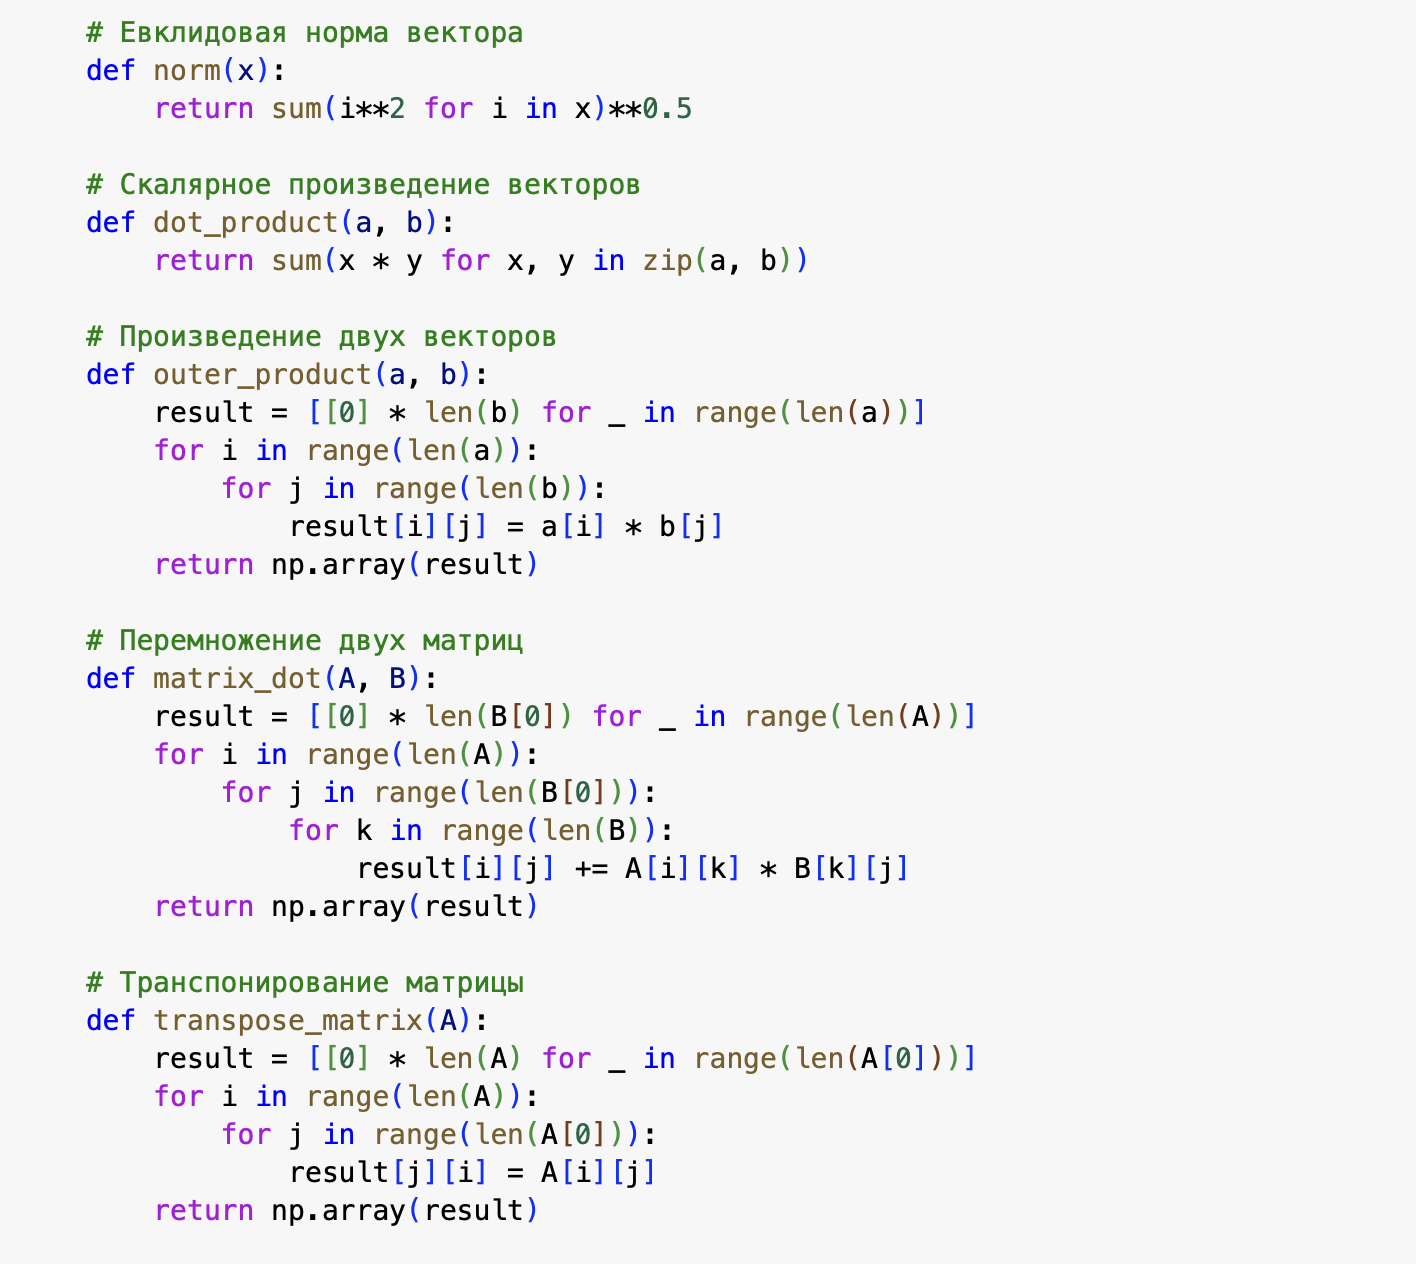
\includegraphics[width=0.7\textwidth]{image1.png}
\end{center}
\end{frame}

\begin{frame}
\frametitle{Реализация основных функций}
\begin{center}
    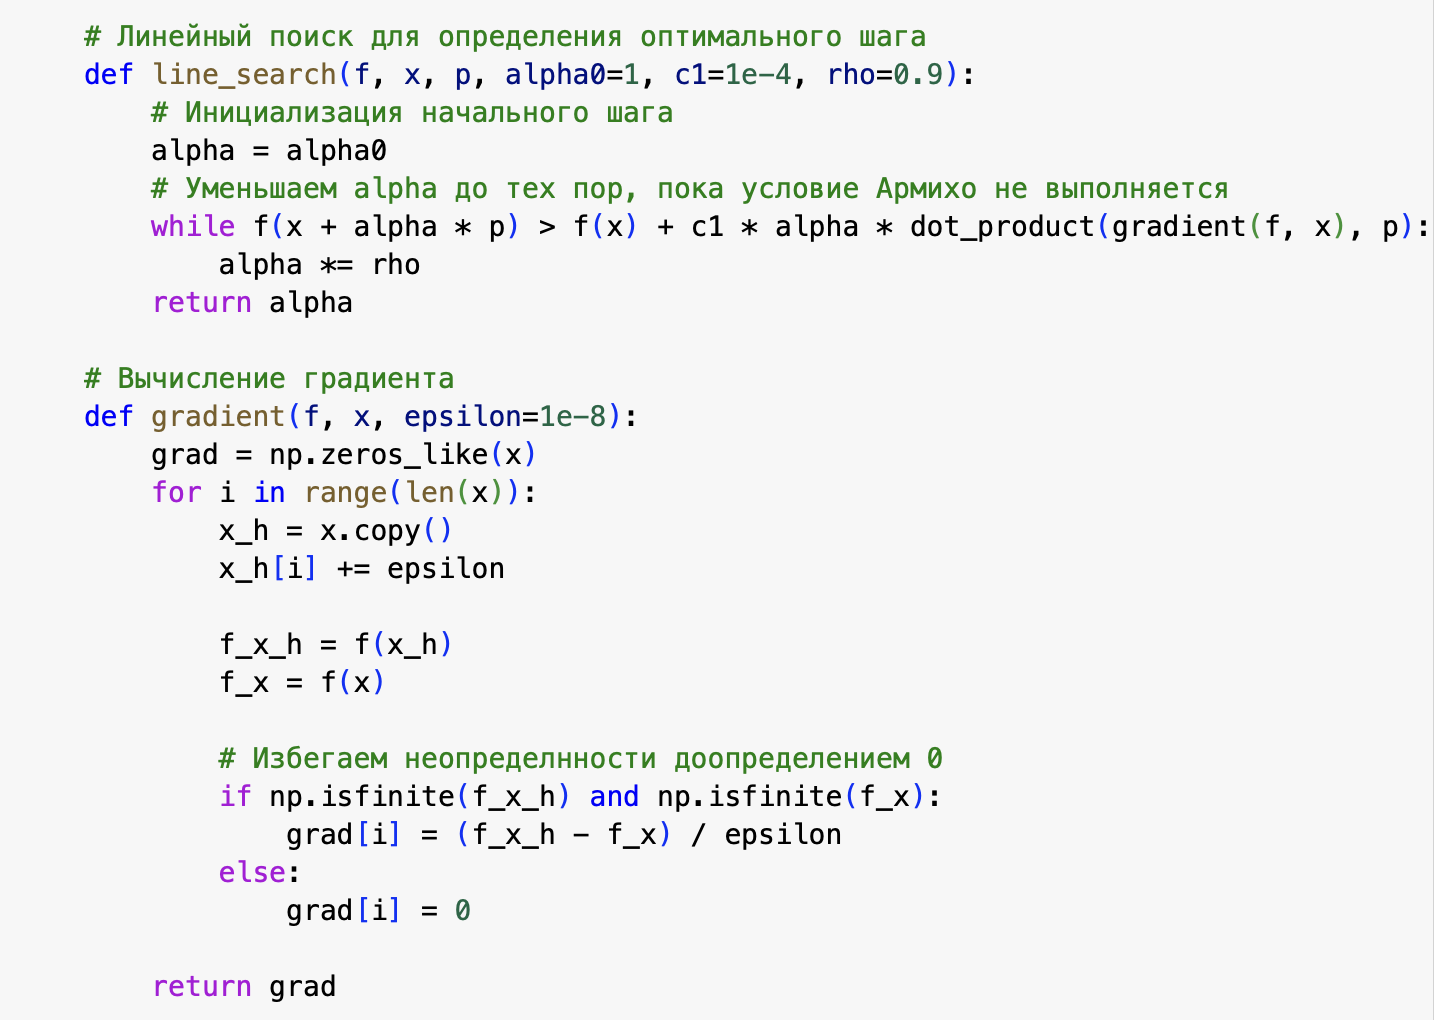
\includegraphics[width=0.9\textwidth]{image2.png}
\end{center}
\end{frame}

\begin{frame}
\frametitle{Реализация барьерной функции}
\begin{center}
    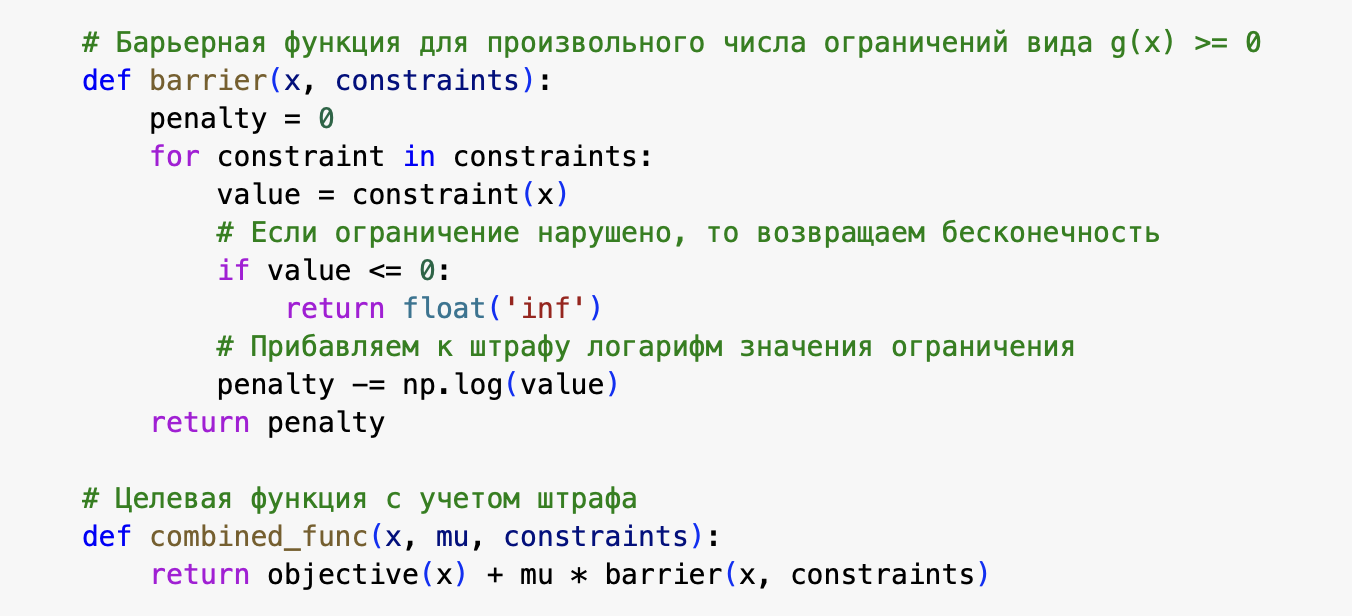
\includegraphics[width=0.9\textwidth]{image3.png}
\end{center}
\end{frame}

\begin{frame}
\frametitle{Реализация DFP с методом барьерных функций}
\begin{center}
    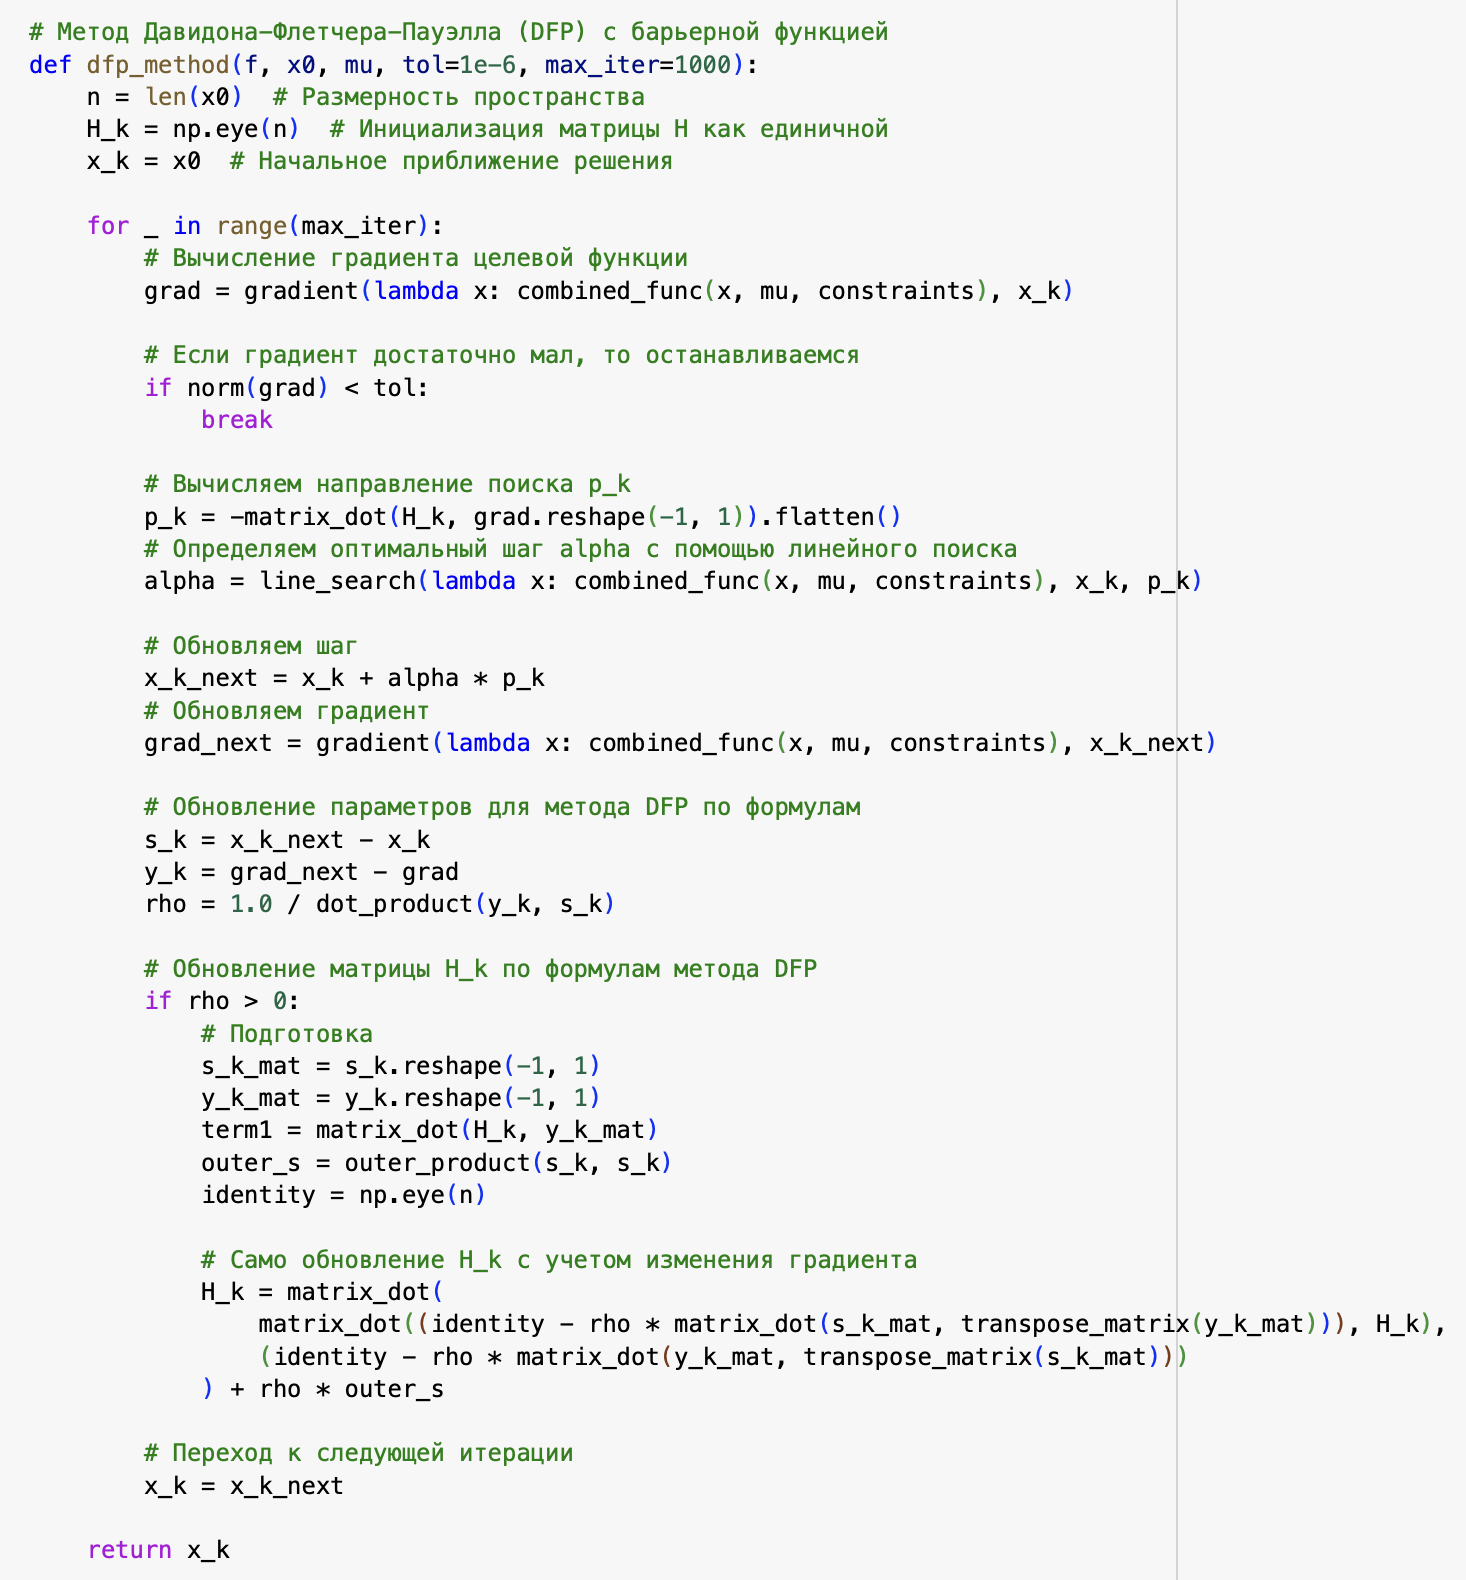
\includegraphics[width=1\textwidth]{image4.png}
\end{center}
\end{frame}

\begin{frame}
\frametitle{Пример 1}
\[
f(x) = (x_0 - 3)^2 + (x_1 - 2)^2
\]
Ограничения: \\
\[
x_0 \geq 1, \quad x_1 \geq 1
\]

Начальная точка: $(2.0, 1.5)$
Оптимальное решение: $(3.0, 2.0)$
Значение целевой функции: $0.0$
\end{frame}

\begin{frame}
\frametitle{Пример 1}
\begin{center}
    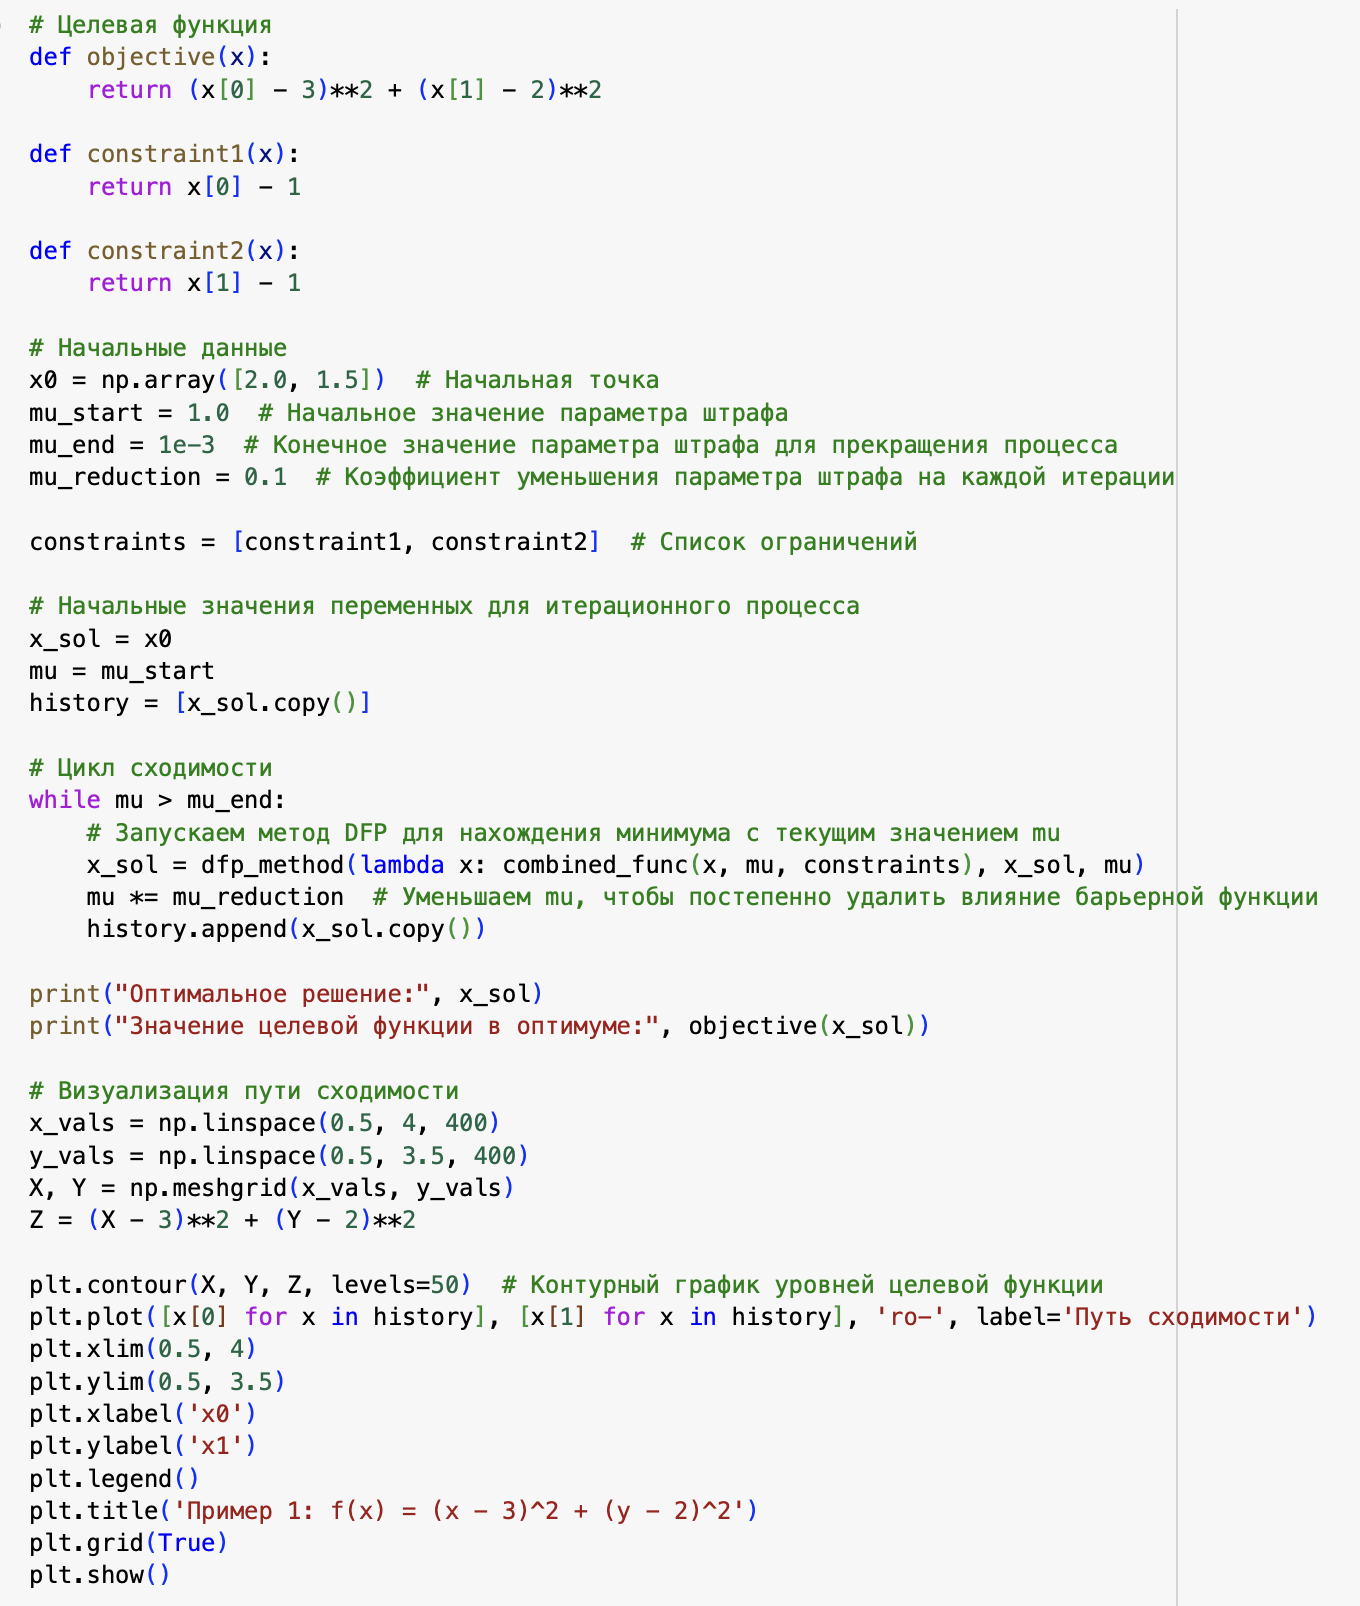
\includegraphics[width=0.6\textwidth]{image5.png}
\end{center}
\end{frame}

\begin{frame}
\frametitle{Пример 1}
\begin{center}
    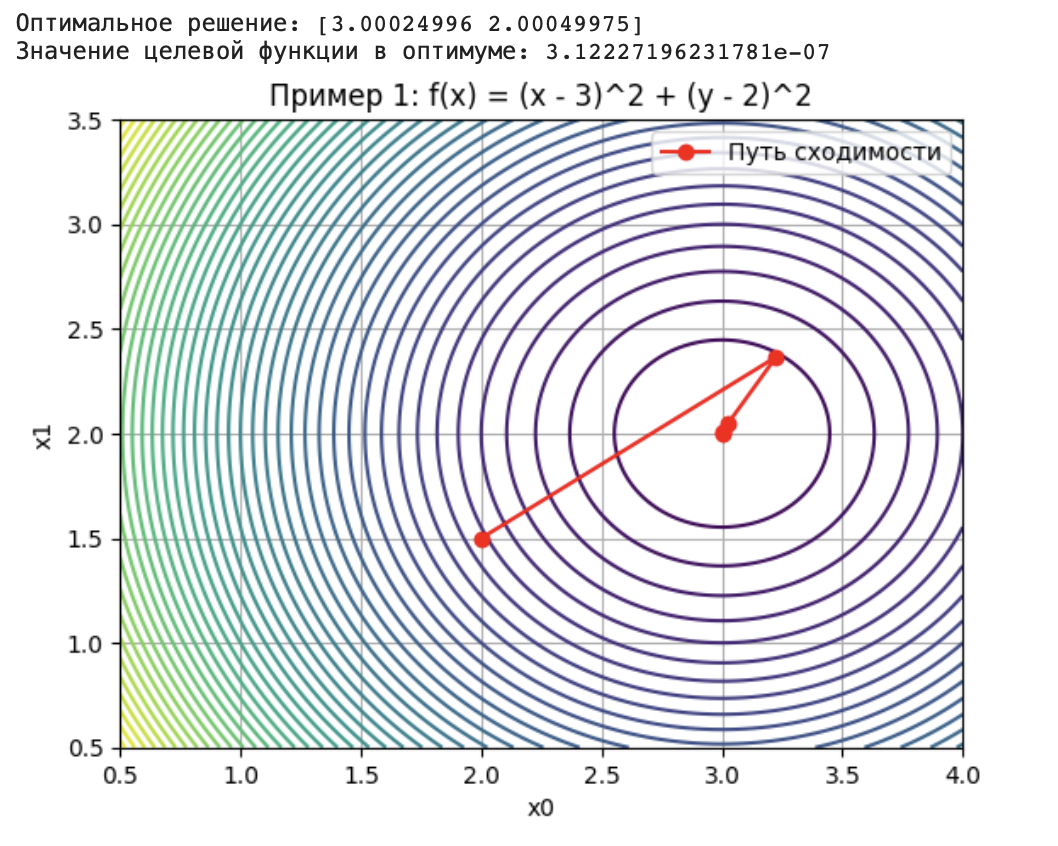
\includegraphics[width=0.8\textwidth]{image6.png}
\end{center}
\end{frame}

\begin{frame}
\frametitle{Пример 2}
\[
f(x) = 2x_0^2 + x_0x_1 + x_1^2
\]
Ограничения: \\
\[
x_0 <= 2, \quad x_1 <= 2
\]
Начальная точка: $(0.5, 1.0)$
Оптимальное решение: $(0.0, 0.0)$
Значение целевой функции: $0.0$
\end{frame}

\begin{frame}
\frametitle{Пример 2}
\begin{center}
    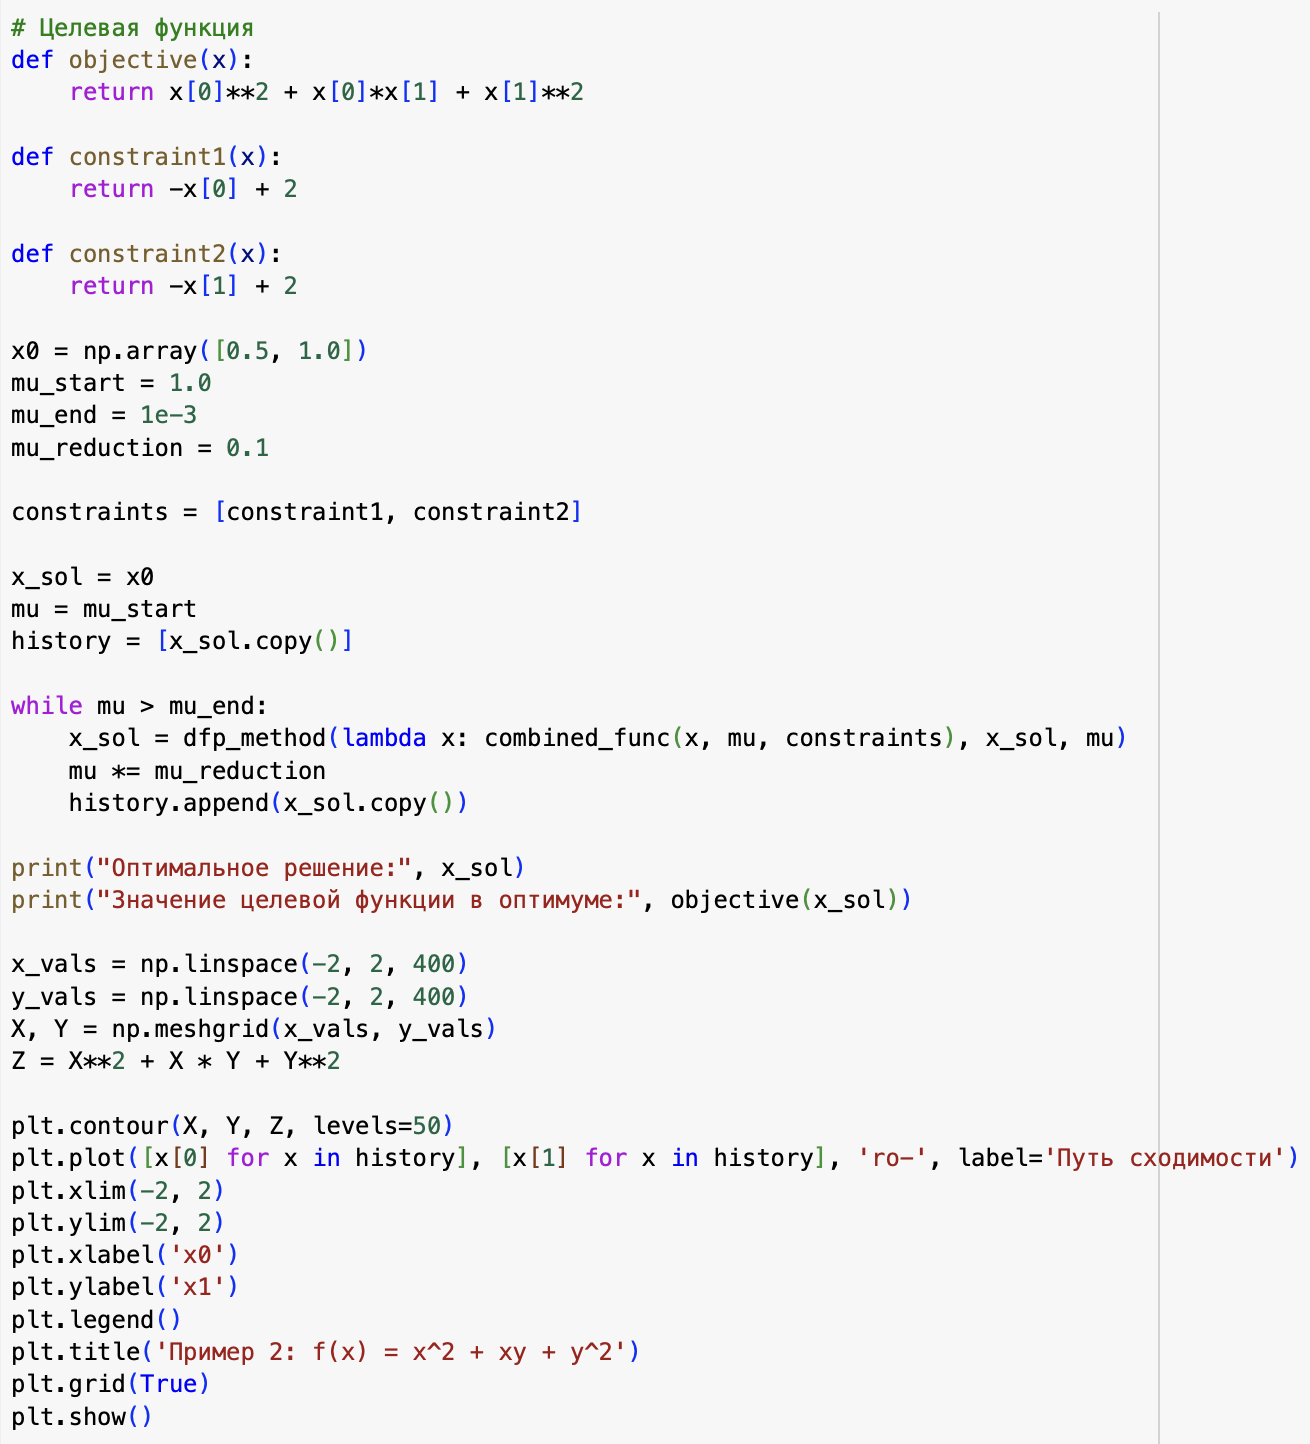
\includegraphics[width=0.6\textwidth]{image7.png}
\end{center}
\end{frame}

\begin{frame}
\frametitle{Пример 2}
\begin{center}
    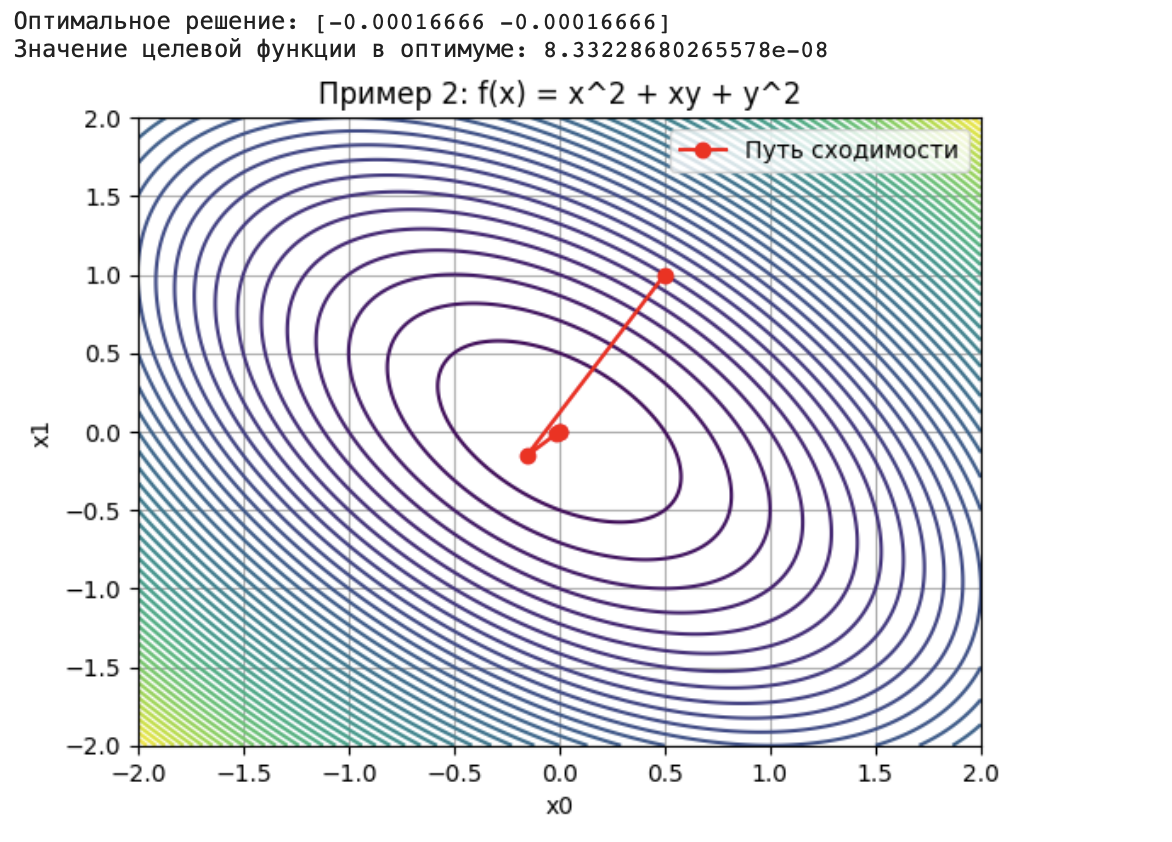
\includegraphics[width=0.8\textwidth]{image8.png}
\end{center}
\end{frame}

\begin{frame}
\frametitle{Пример на выданных функциях}
Выданная целевая функция: \\
\[
f(x) = \sum_{i=1}^4((x_i - 7)^2 + 42(x_{i+1} - x_i^2)^2)
\]

Барьерная функция: \\
\[
g(x) = \sum_{i=1}^5(i*x_i^2) \leqslant 72
\]

\end{frame}

\begin{frame}
\frametitle{Результат работы стандартных питоновских функций}
\begin{center}
    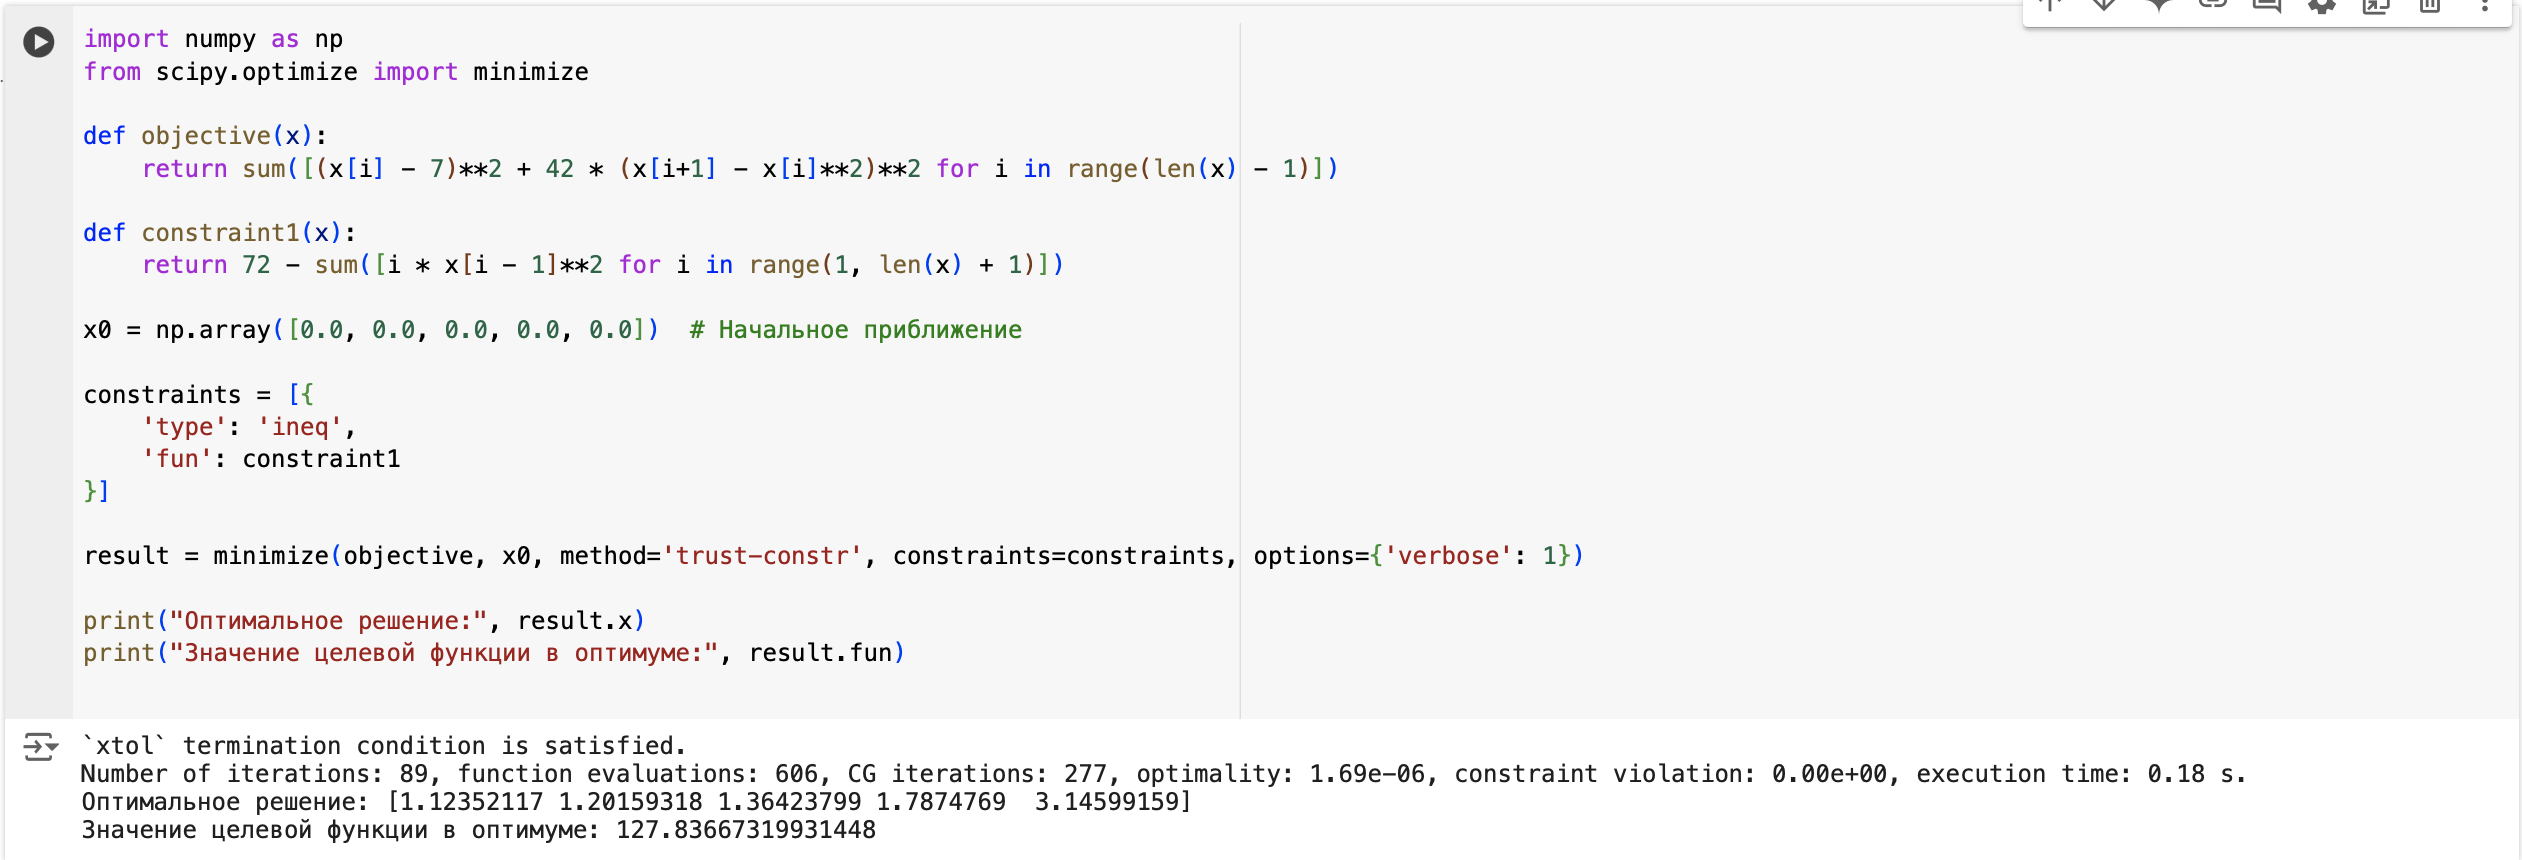
\includegraphics[width=1\textwidth]{python_optim_const.png}
\end{center}
Оптимальное решение: [1.12352117 1.20159318 1.36423799 1.7874769  3.14599159]
Значение целевой функции в оптимуме: 127.83667319931448
\end{frame}

\begin{frame}
\frametitle{Результат работы реализованного DFP метода с барьерной функцией}
\begin{center}
    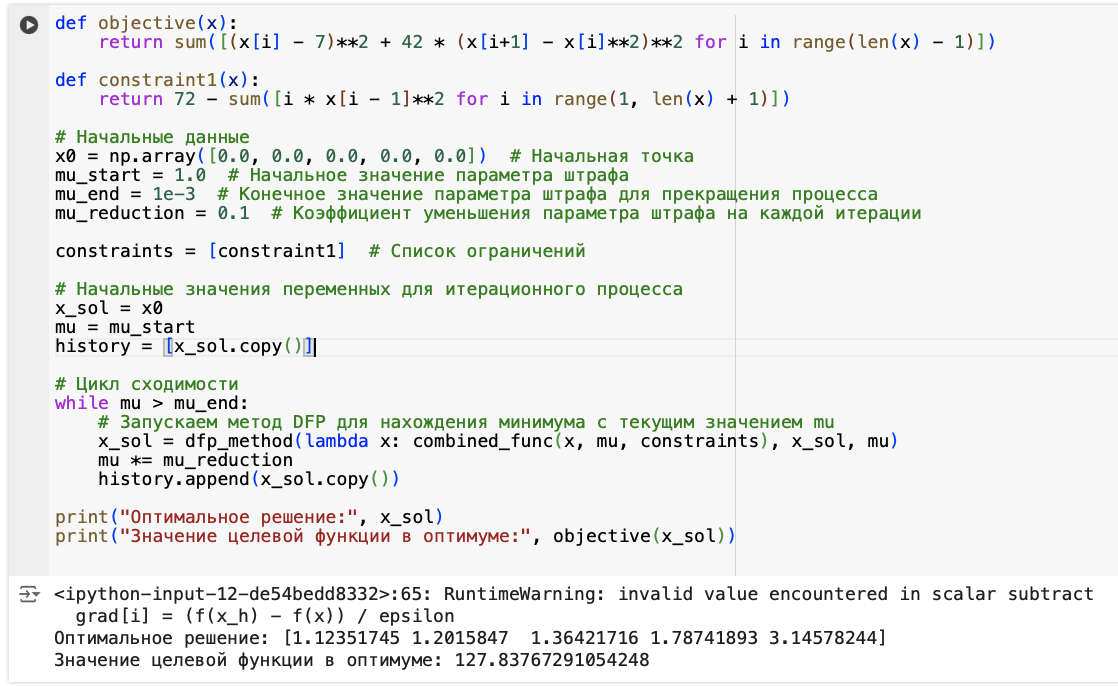
\includegraphics[width=1\textwidth]{my_optim.png}
\end{center}
\end{frame}

\begin{frame}
\frametitle{Результат работы стадартных питоновских функций без ограничений}
\begin{center}
    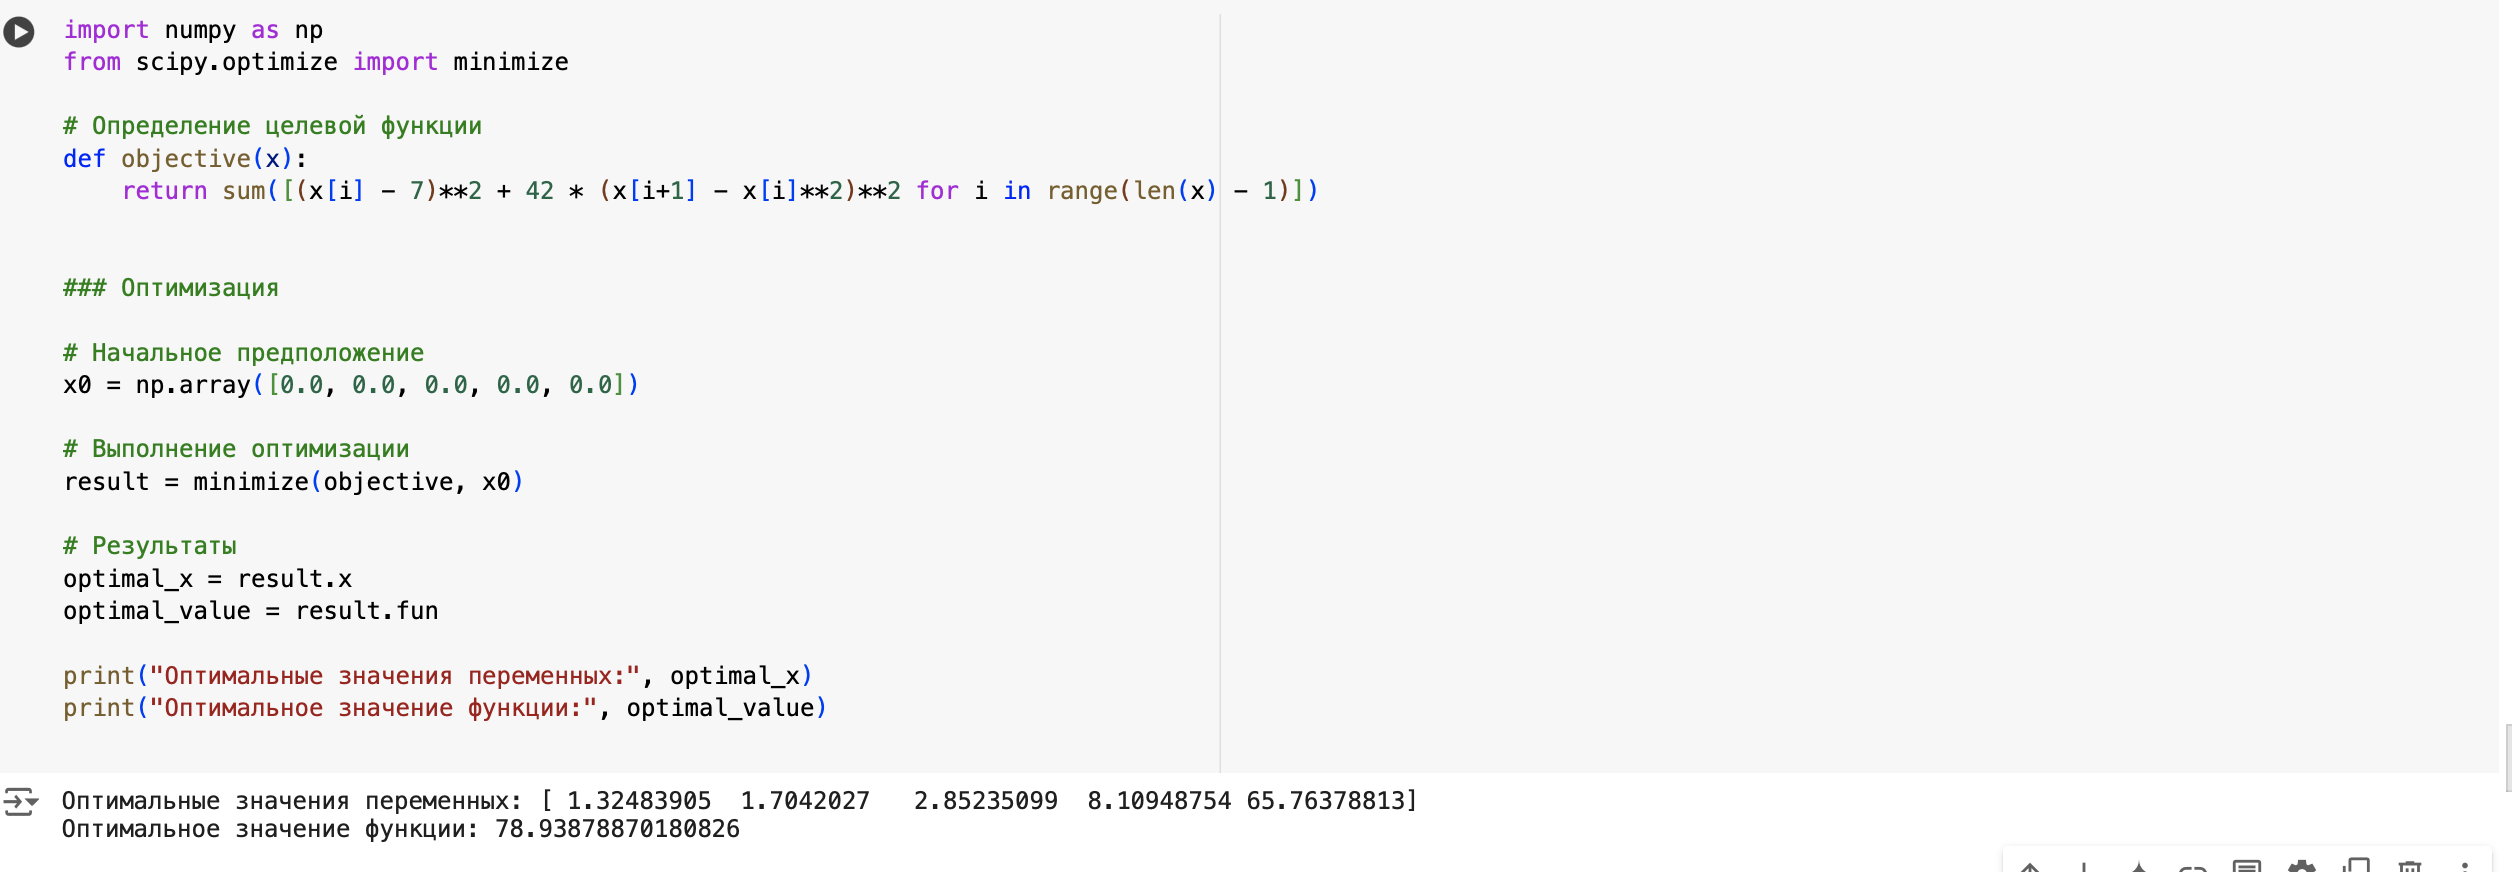
\includegraphics[width=1\textwidth]{python_optim.png}
\end{center}
Оптимальные значения переменных: [ 1.32483905  1.7042027   2.85235099  8.10948754 65.76378813]
Оптимальное значение функции: 78.93878870180826
\end{frame}

\begin{frame}
\frametitle{Результат работы реализованного DFP метода с увеличенной барьерной функцией}
\begin{center}
    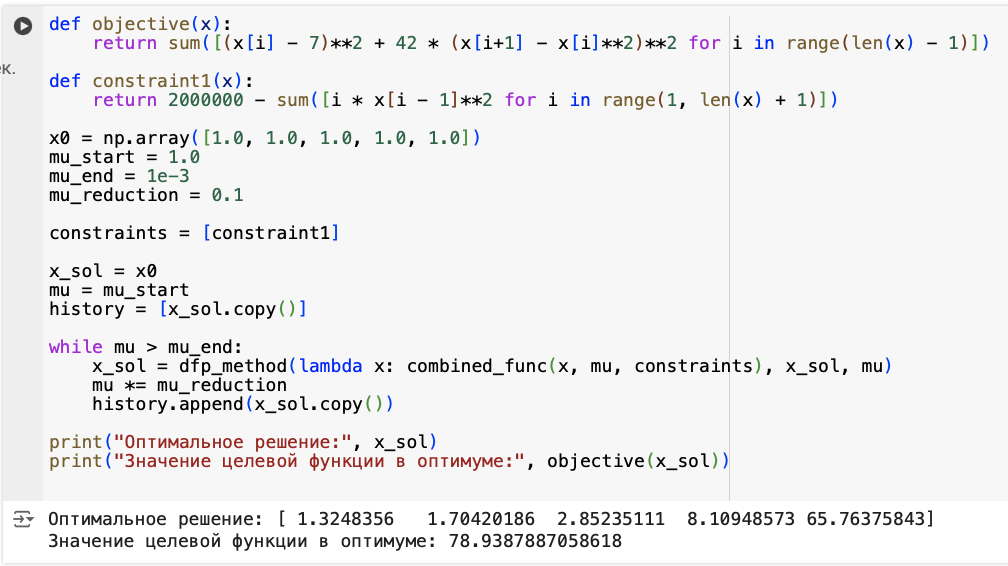
\includegraphics[width=1\textwidth]{my_optim_const.png}
\end{center}
\end{frame}

\begin{frame}
\frametitle{Выводы}
Насколько видно из проведенных экспериментов глобальное оптимальное решение xt = [ 1.32483905  1.7042027   2.85235099  8.10948754 65.76378813]
$g(xt) = \sum_{i=1}^5(i*x_i^2) = 21918 > 72$
для выданной целевой функции f(x) находится за пределами выданной барьерной функции g(x), поэтому программа выдает с точностью 0.001 локальное оптимальное решение на доступном для нее пространстве (сверяем со стандартной питоновской выдачей). Если увеличить g(x) до <= 21920 и более, то программа выдает с точностью 0.00000001 верное глобальное оптимальное решение (также сверяем со стандартными питоновскими методами оптимизации). 
\end{frame}

\begin{frame}
\frametitle{зависимость числа итераций от (x0, 0, 0, 0, 0) }
\begin{center}
    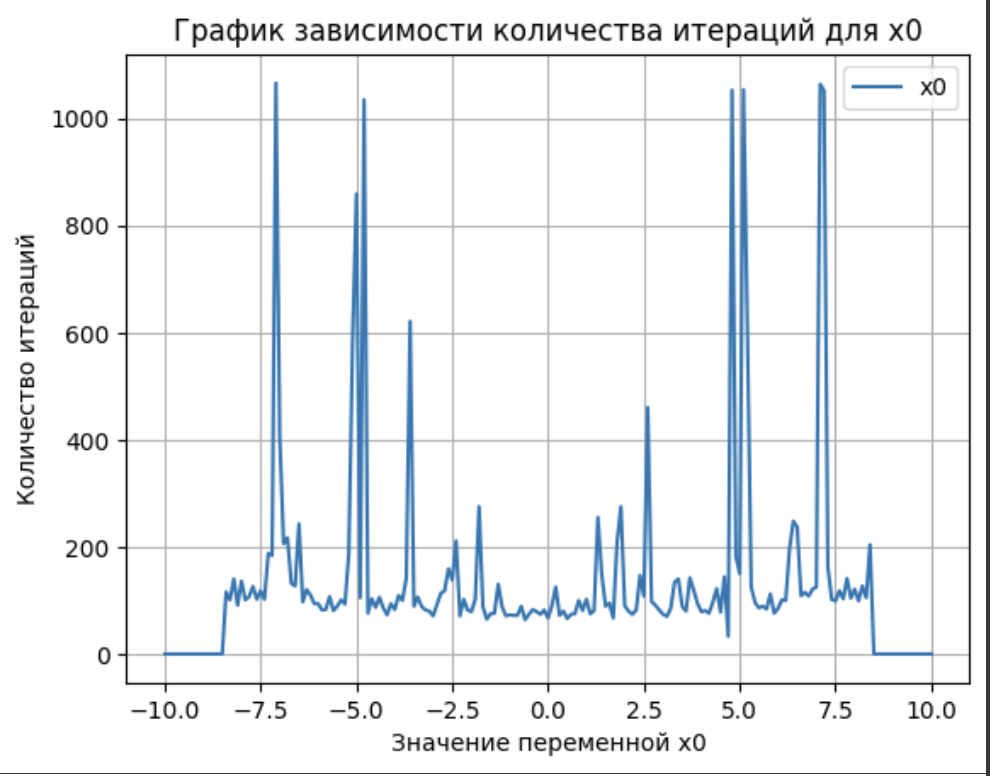
\includegraphics[width=0.8\textwidth]{x0.png}
\end{center}
\end{frame}

\begin{frame}
\frametitle{зависимость числа итераций от (0, x1, 0, 0, 0) }
\begin{center}
    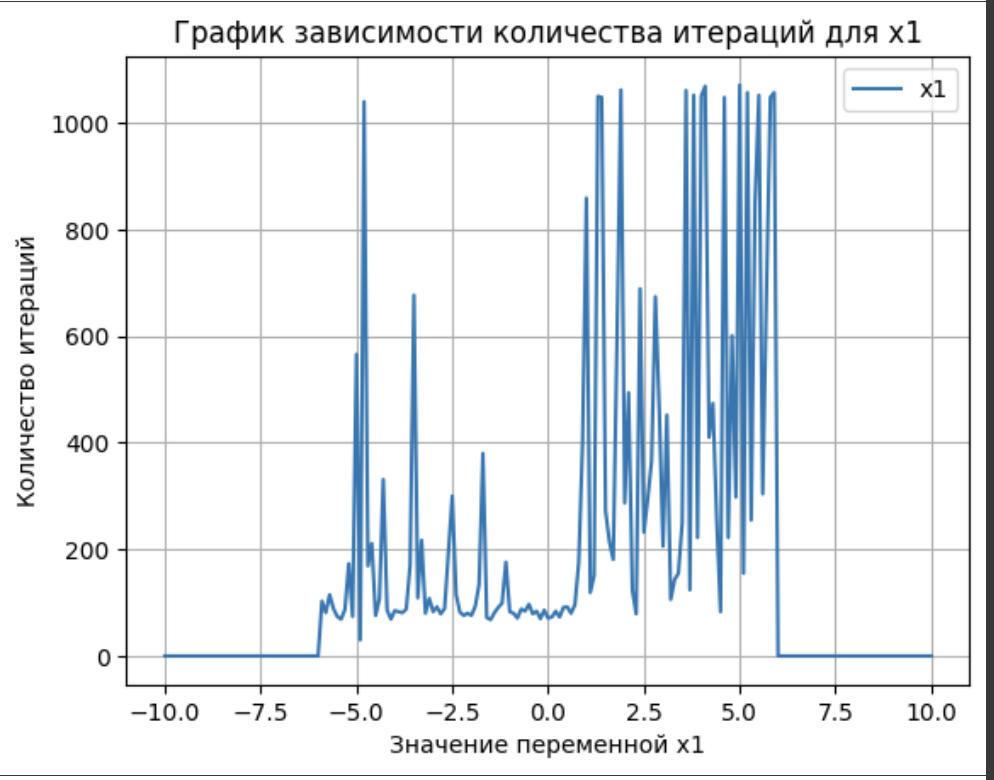
\includegraphics[width=0.8\textwidth]{x1.png}
\end{center}
\end{frame}

\begin{frame}
\frametitle{зависимость числа итераций от (0, 0, x2, 0, 0) }
\begin{center}
    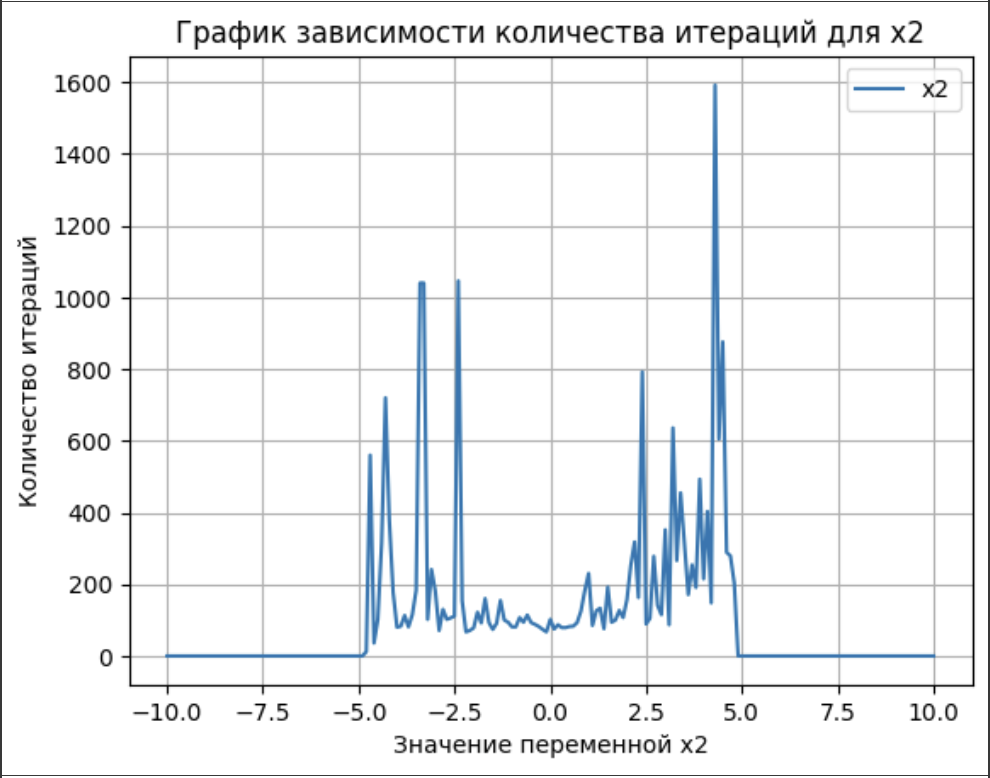
\includegraphics[width=0.8\textwidth]{x2.png}
\end{center}
\end{frame}

\begin{frame}
\frametitle{зависимость числа итераций от (0, 0, 0, x3, 0) }
\begin{center}
    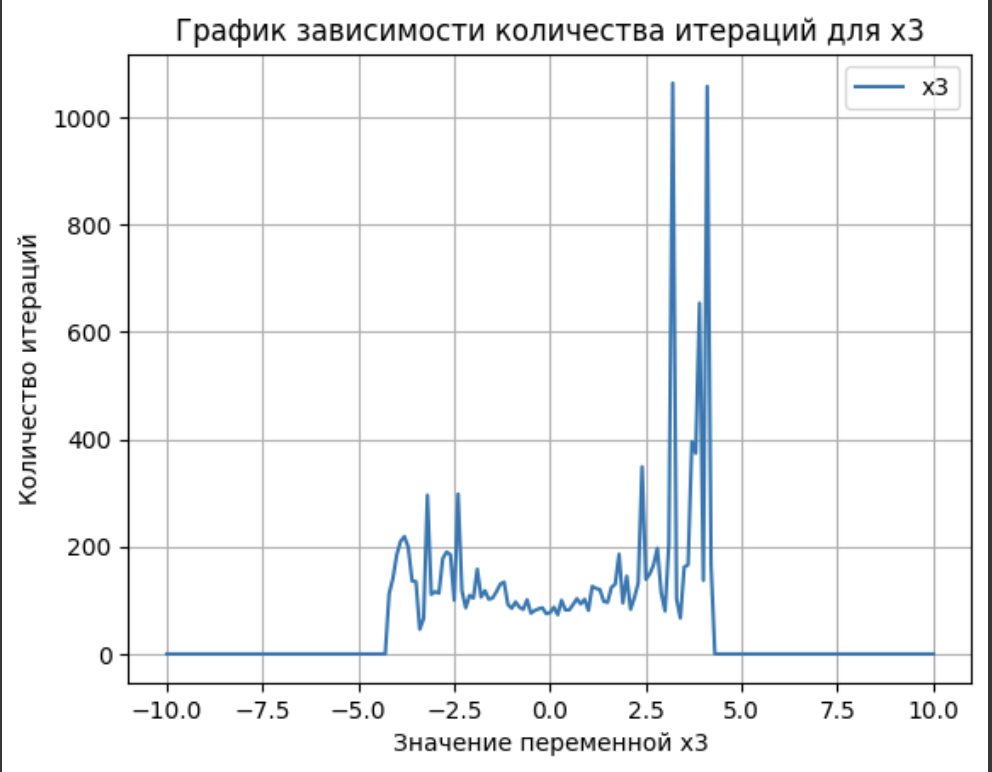
\includegraphics[width=0.8\textwidth]{x3.png}
\end{center}
\end{frame}

\begin{frame}
\frametitle{зависимость числа итераций от (0, 0, 0, 0, x4) }
\begin{center}
    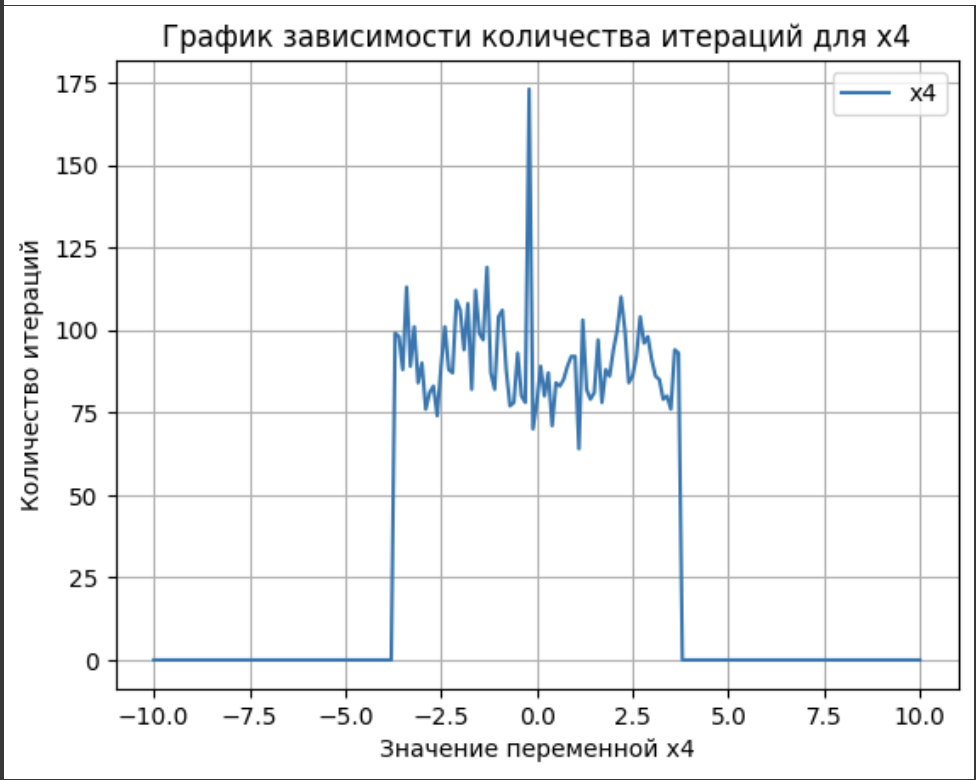
\includegraphics[width=0.8\textwidth]{x4.png}
\end{center}
\end{frame}

\begin{frame}
\frametitle{таблица решений в зависимости от выбора начальной точки вида (x,x,x,x)}
\begin{center}
    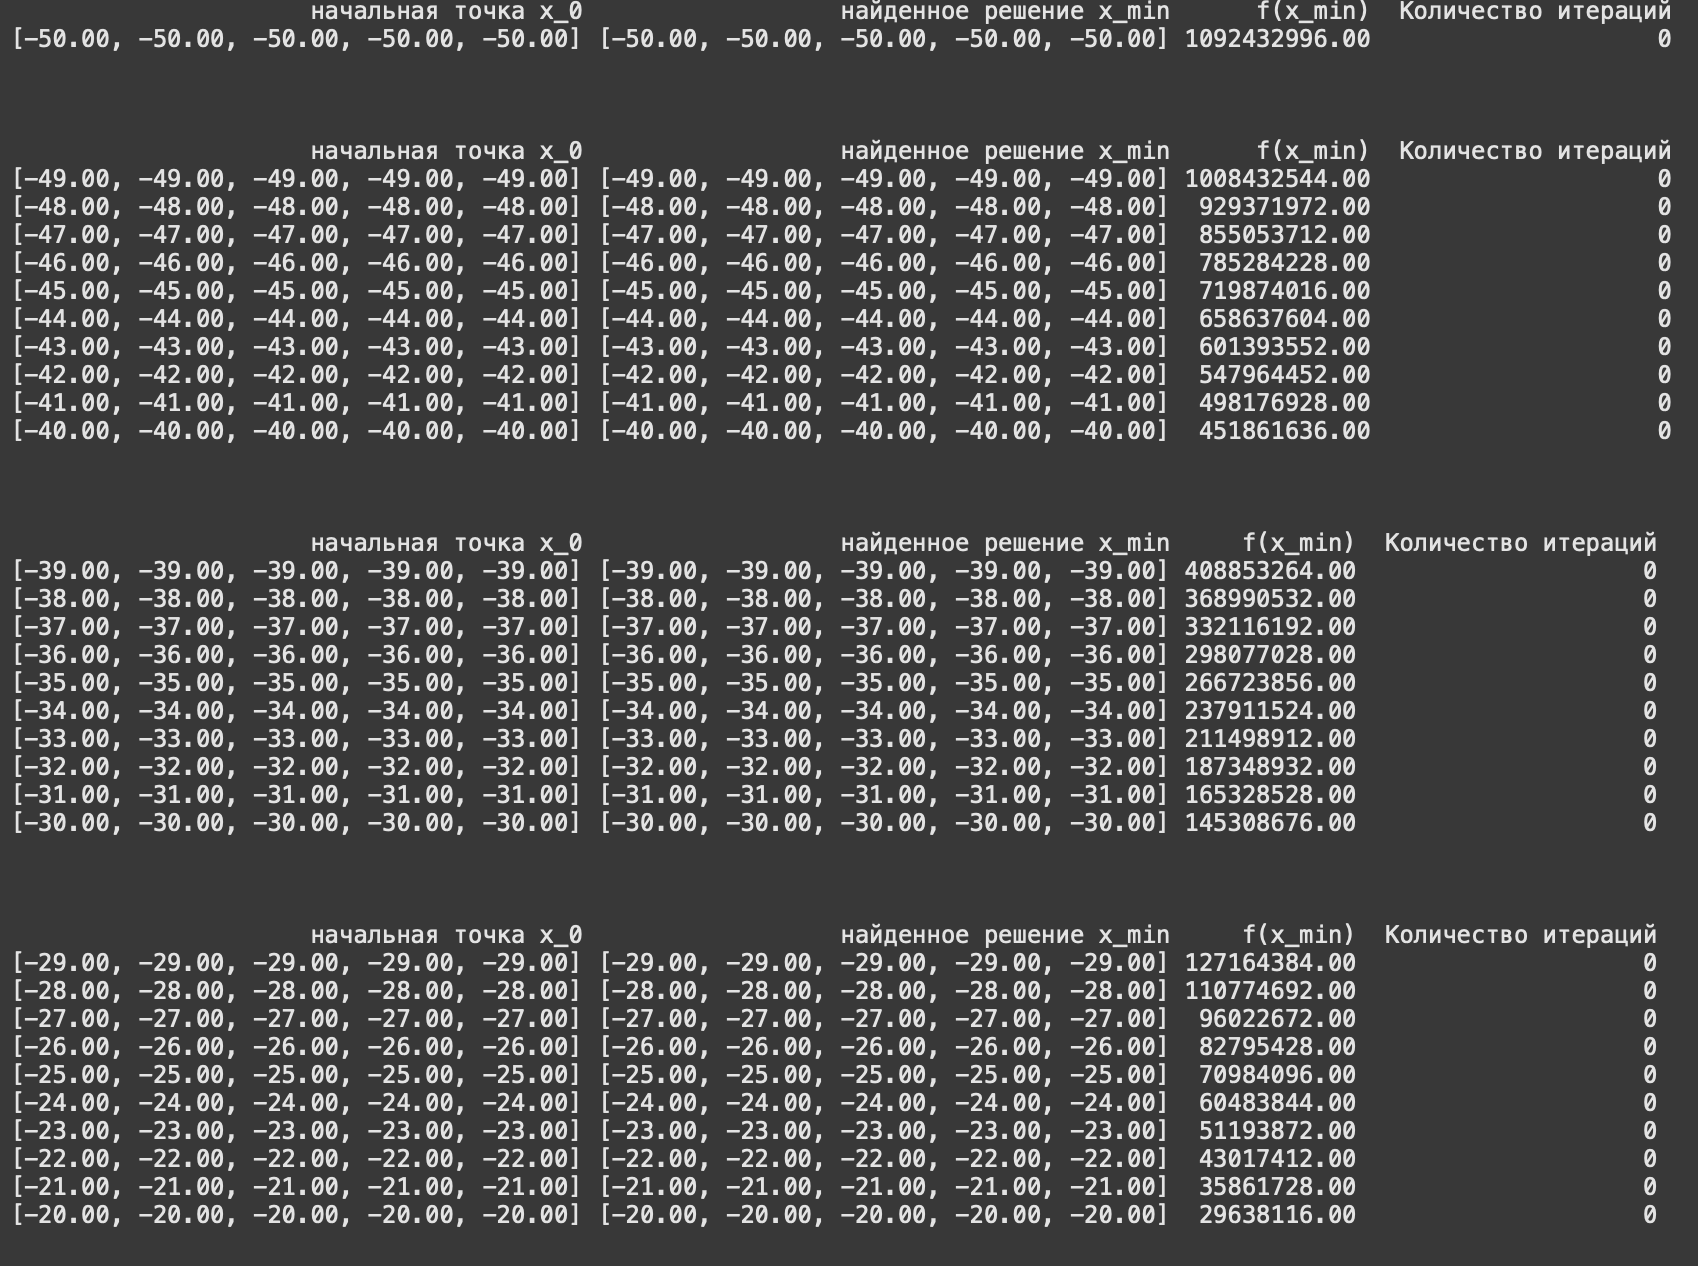
\includegraphics[width=0.8\textwidth]{xxx1.png}
\end{center}

\end{frame}

\begin{frame}
\frametitle{таблица решений в зависимости от выбора начальной точки вида (x,x,x,x)}
\begin{center}
    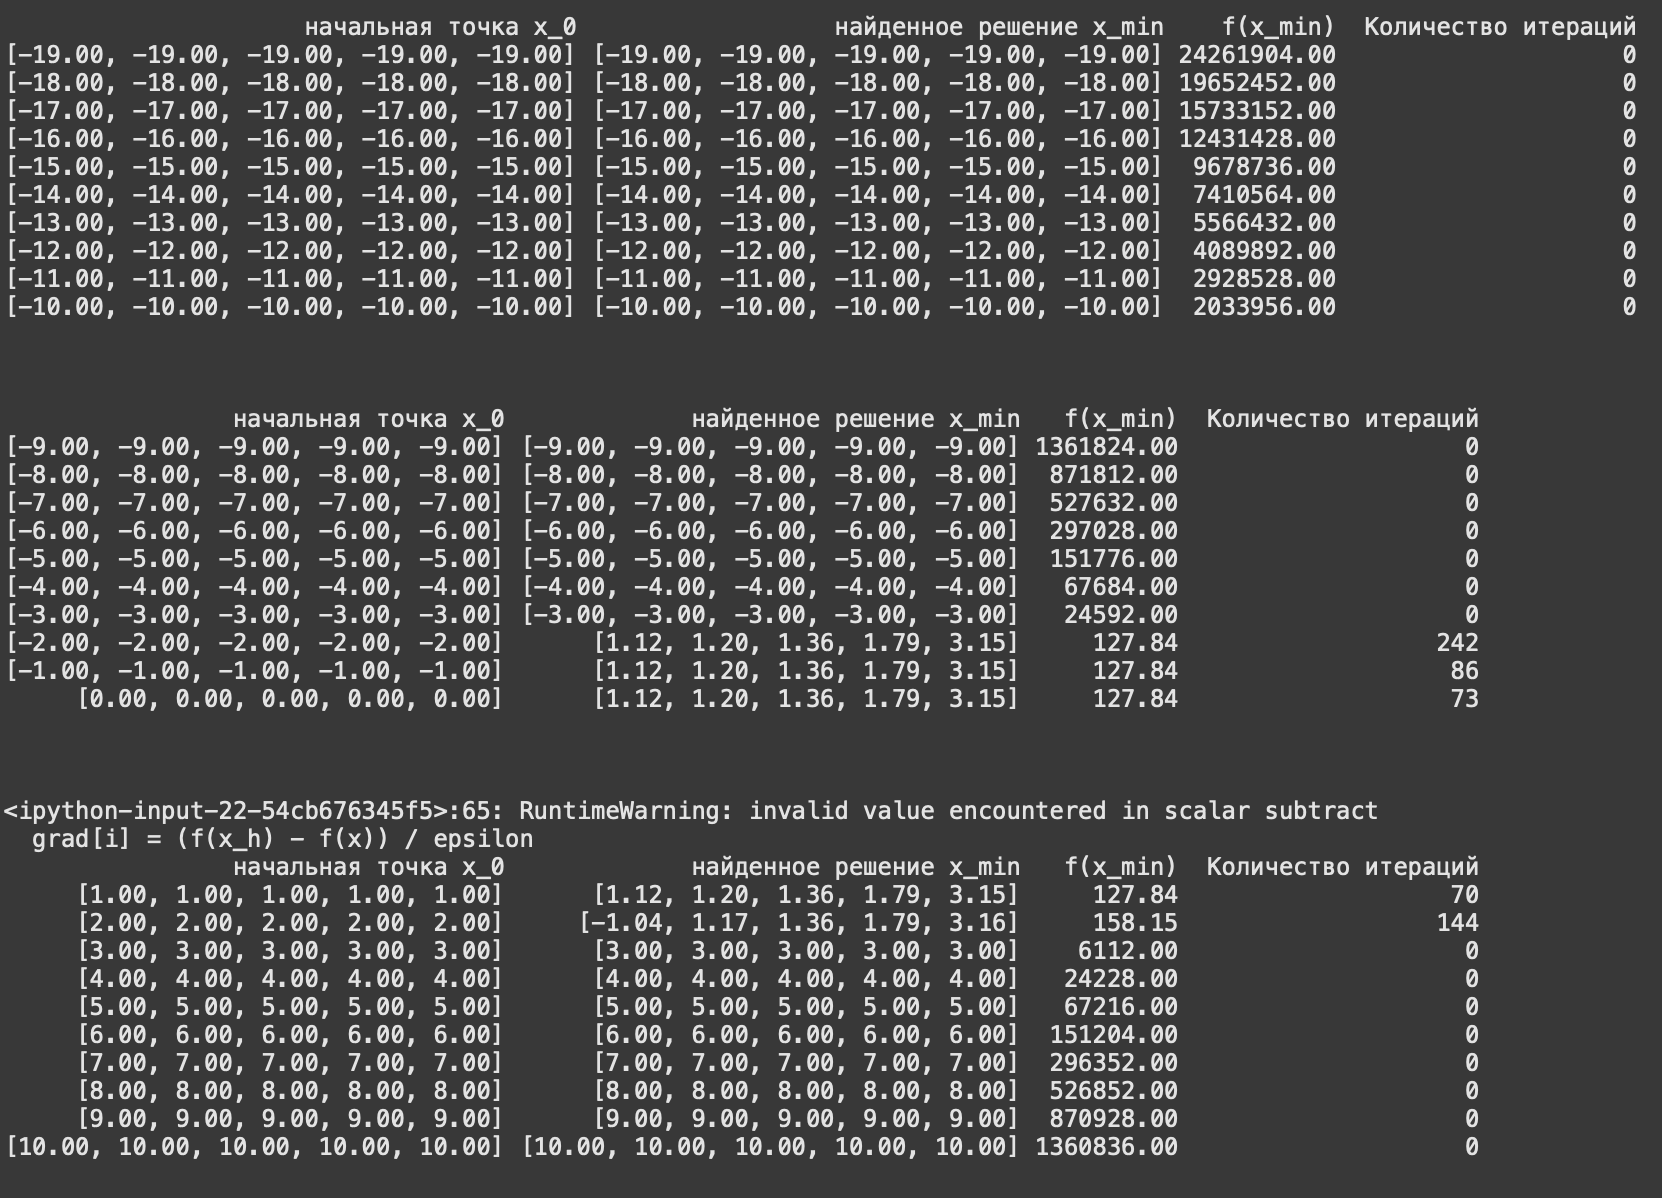
\includegraphics[width=0.8\textwidth]{xxx2.png}
\end{center}
\end{frame}

\begin{frame}
\frametitle{таблица решений в зависимости от выбора начальной точки вида (x,x,x,x)}
\begin{center}
    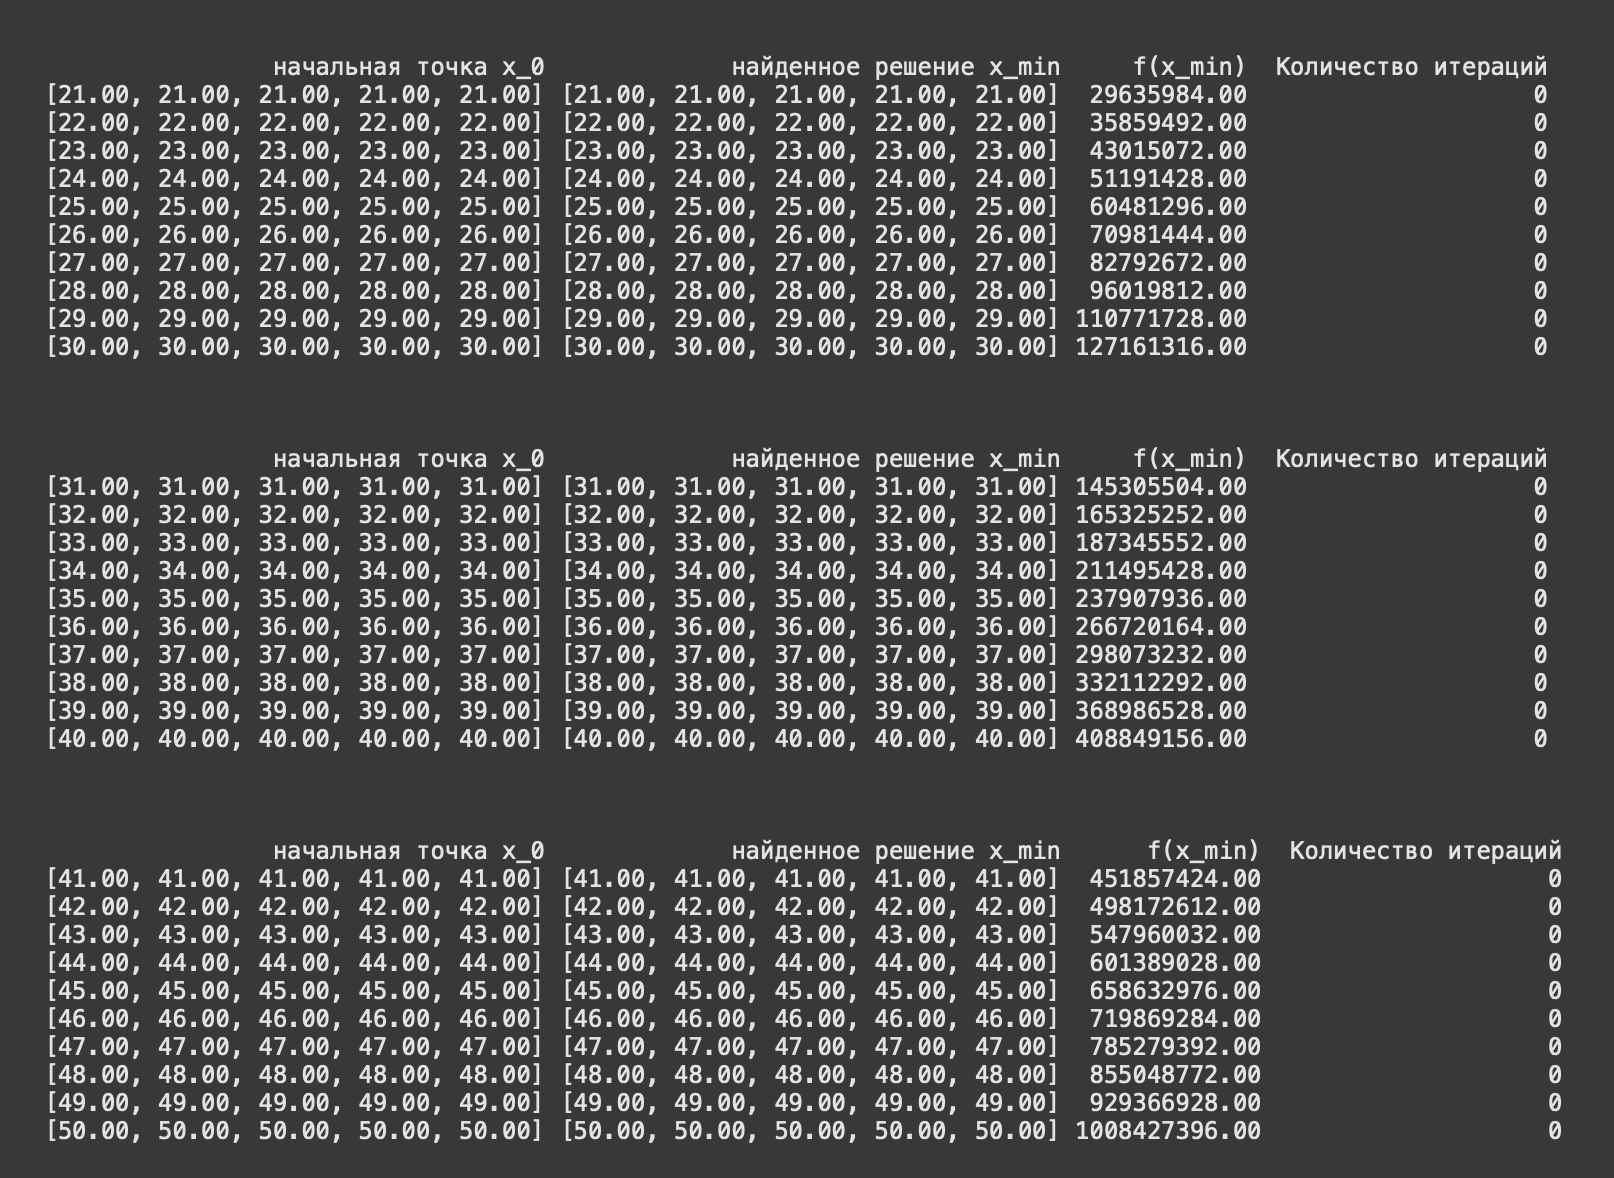
\includegraphics[width=0.8\textwidth]{xxx3.png}
\end{center}

\end{frame}

\begin{frame}
\frametitle{Вывод}
Где 0 итераций, значит метод не сходится. Исходя из полученных данных, можно сказать, что метод сходится с достаточной точностью и за приемлимое число итераций из точки-окрестности нуля диаметра (-2.5, 2.5).

\end{frame}

\begin{frame}
\frametitle{таблицу решений в зависимости от изменения радиуса допустимой области}
\begin{center}
    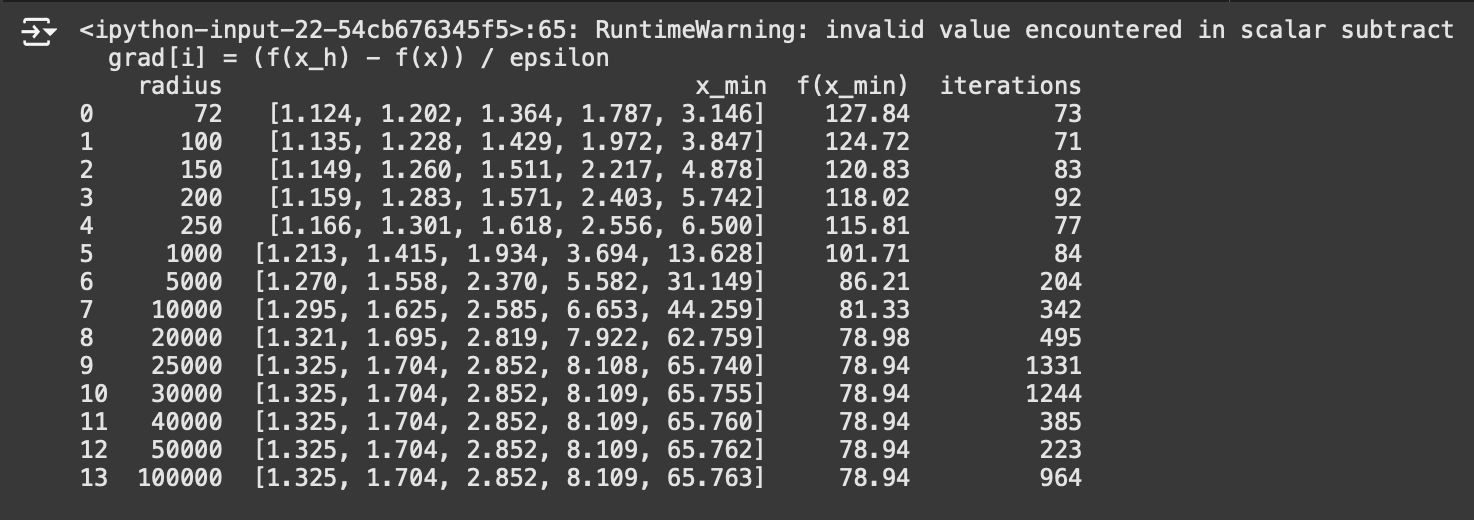
\includegraphics[width=0.8\textwidth]{radius.png}
\end{center}

\end{frame}

\begin{frame}
\frametitle{Выводы}
Насколько видно из проведенных экспериментов глобальное оптимальное решение xt = [ 1.32483905  1.7042027   2.85235099  8.10948754 65.76378813]
$g(xt) = \sum_{i=1}^5(i*x_i^2) = 21918 > 72$
для выданной целевой функции f(x) находится за пределами выданной барьерной функции g(x), поэтому программа выдает с точностью 0.001 локальное оптимальное решение на доступном для нее пространстве (сверяем со стандартной питоновской выдачей). Если увеличить g(x) до <= 21900 и более, то программа выдает с точностью 0.00000001 верное глобальное оптимальное решение (также сверяем со стандартными питоновскими методами оптимизации). 
\end{frame}

\begin{frame}
\frametitle{ зависимость точности найденного решения от выбора точности критерия остановки}
\begin{center}
    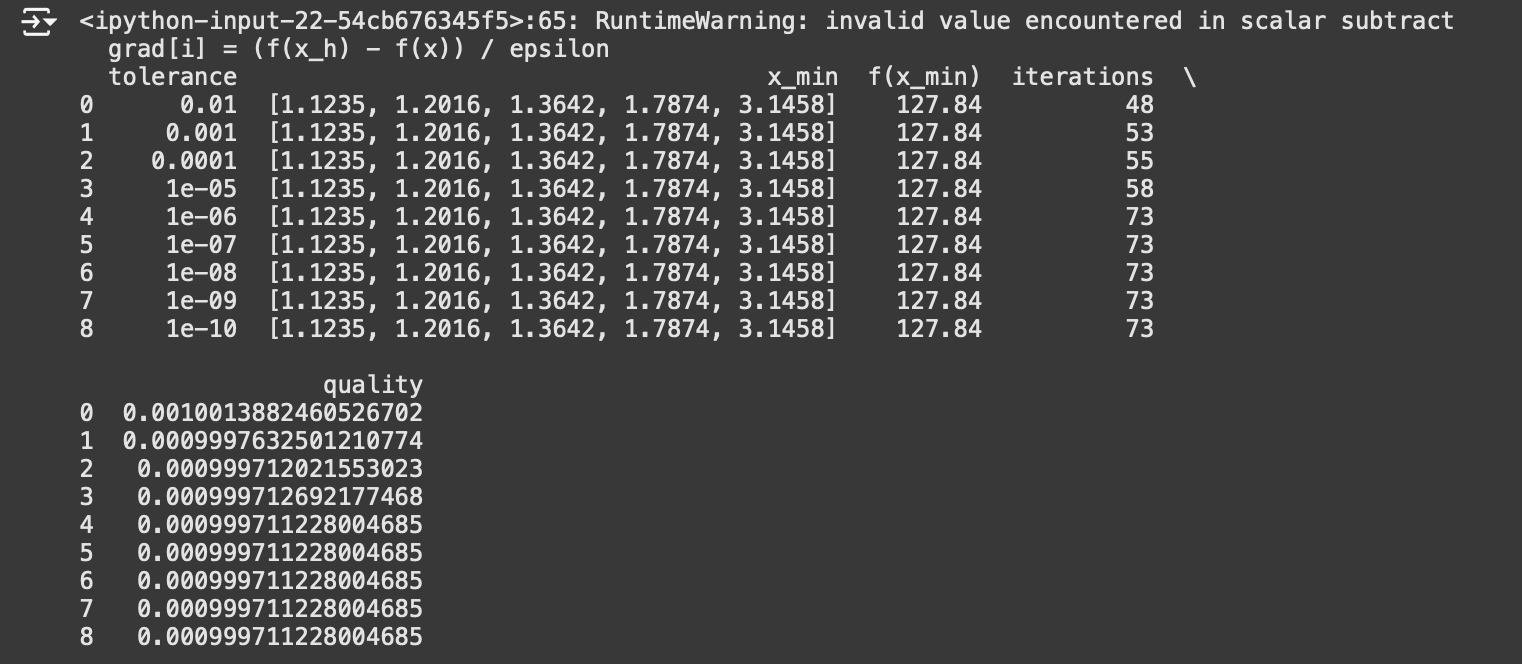
\includegraphics[width=0.8\textwidth]{tolerance.png}
\end{center}

Чем меньше критерий остановки, тем выше точность решения. (точность решения сверяется с решением из стандартных питоновских функций)
\end{frame}

\begin{frame}
\frametitle{Исследовать зависимость числа итераций от длины шага метода при заданной точности 0,0001}
\begin{center}
    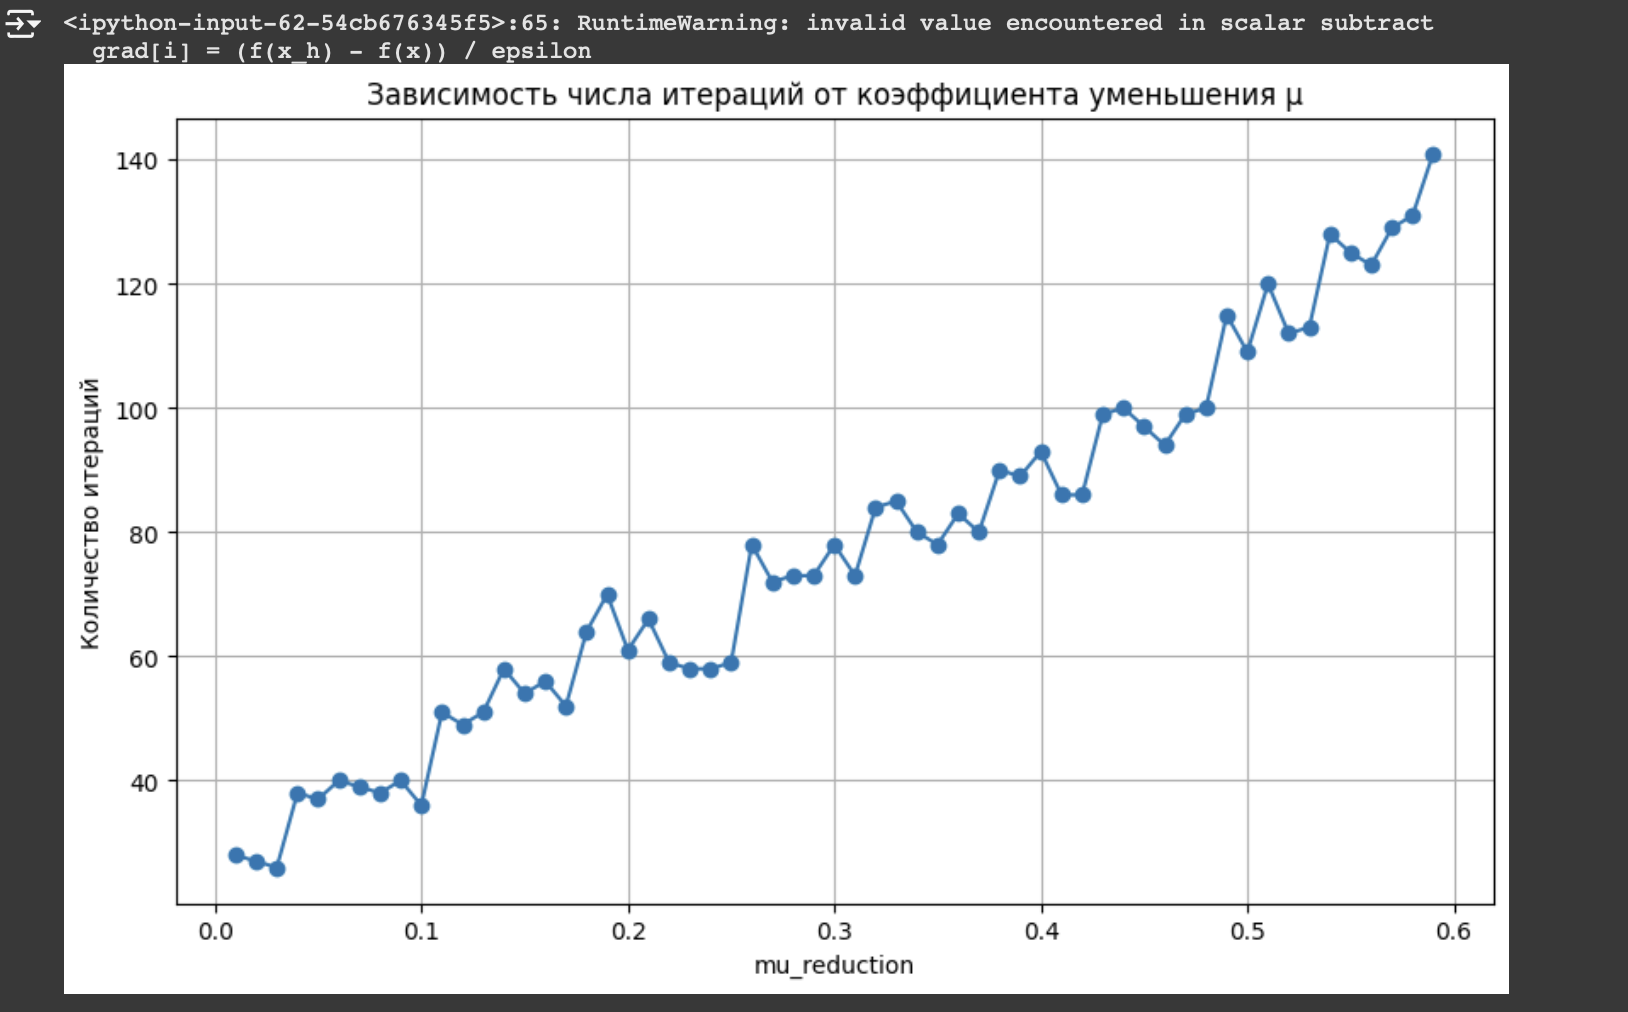
\includegraphics[width=0.8\textwidth]{mu.png}
\end{center}

\end{frame}

\begin{frame}
\frametitle{Исследовать влияние вида барьерной/штрафной функции на скорость сходимости метода}
\begin{center}
    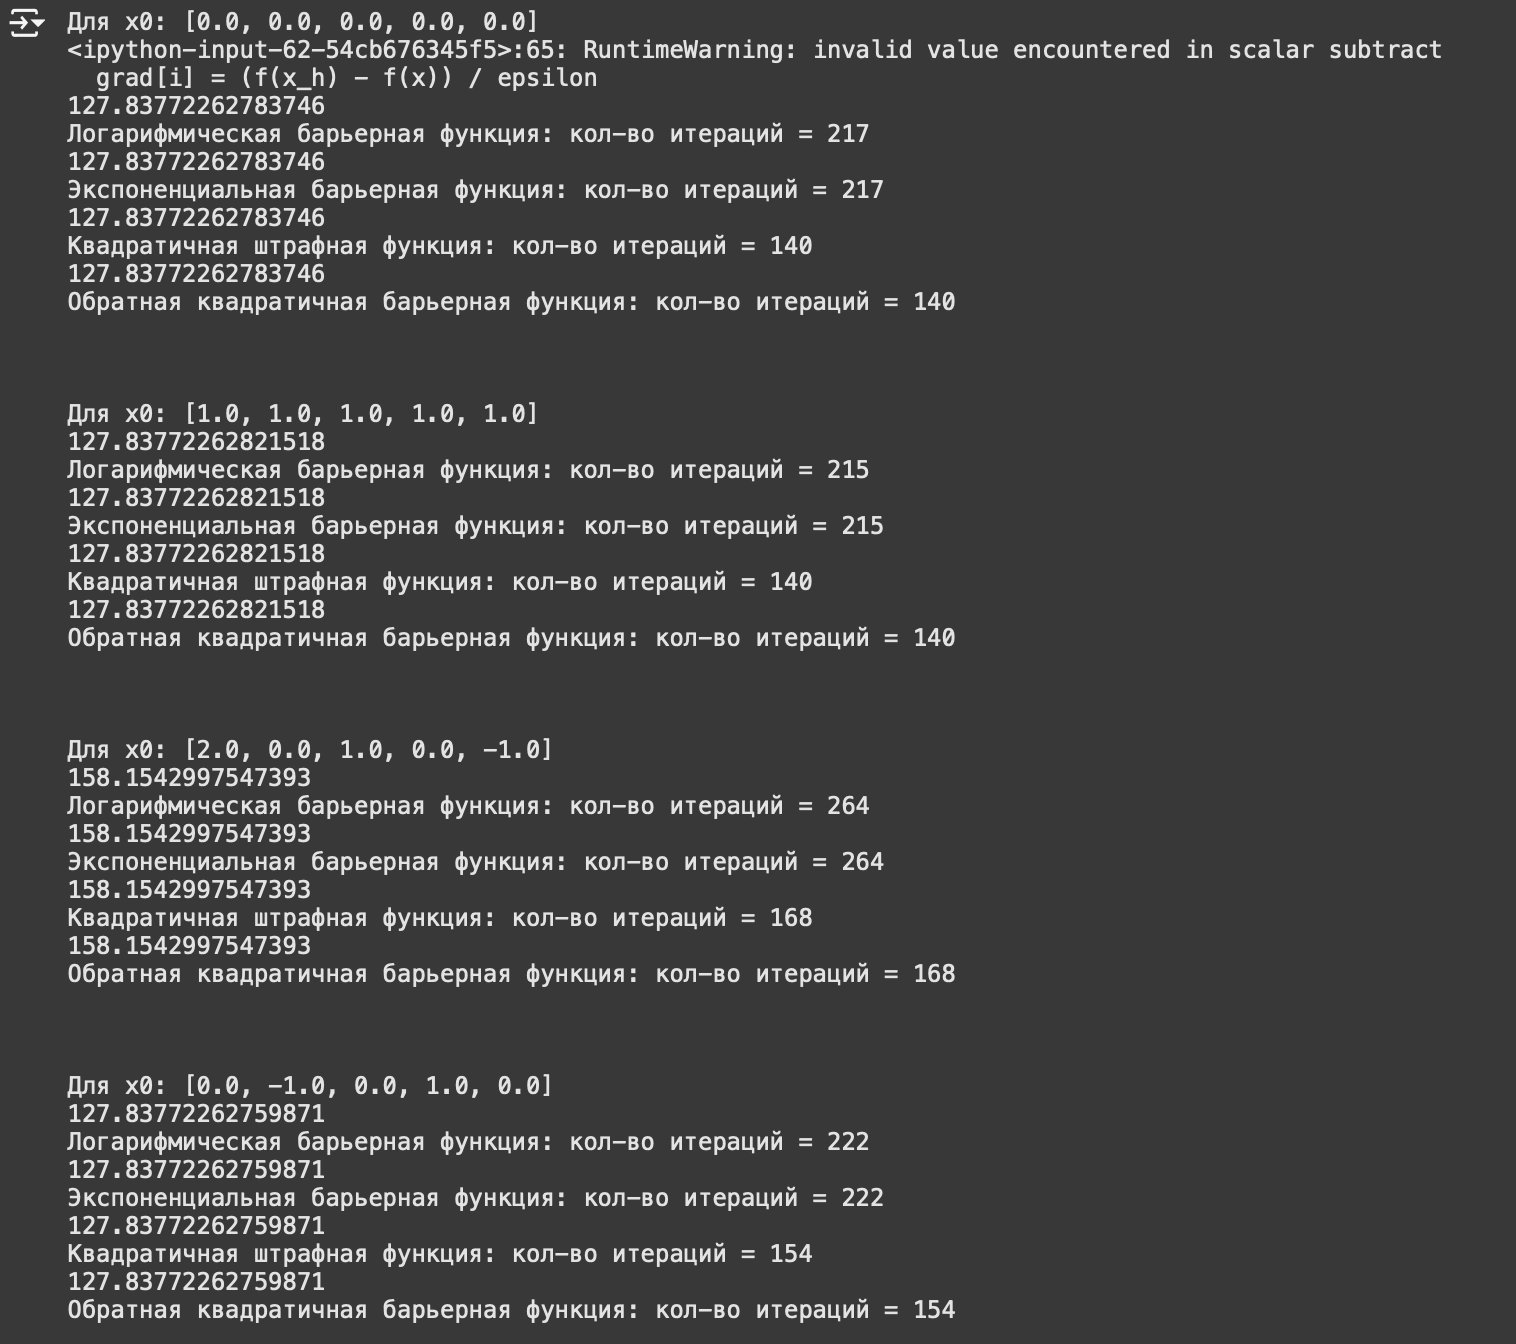
\includegraphics[width=0.6\textwidth]{barrier.png}
\end{center}

\end{frame}

\begin{frame}
\frametitle{Исследовать влияние вида барьерной/штрафной функции на скорость сходимости метода вывод}
Из результатов эксперимента видно, что квадратичная барьерная функция лучше себя показывает по количеству итераций, нежели логарифмическая. Причем в точности не уступает ни одна ни вторая.
\end{frame}

\begin{frame}
\frametitle{ зависимость точности найденного решения от выбора критерия остановки}
\begin{center}
    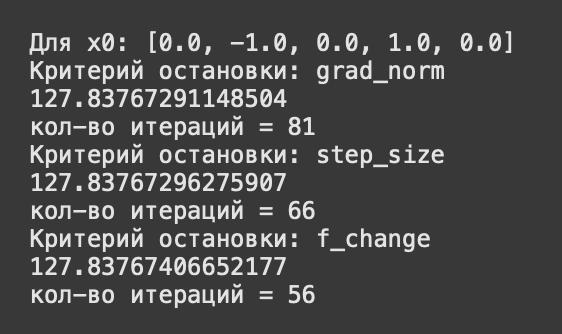
\includegraphics[width=0.8\textwidth]{stop1.png}
\end{center}
\end{frame}

\begin{frame}
\frametitle{ зависимость точности найденного решения от выбора критерия остановки}
\begin{center}
    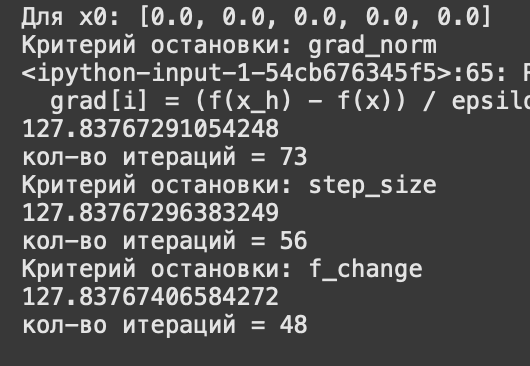
\includegraphics[width=0.8\textwidth]{stop2.png}
\end{center}
\end{frame}

\begin{frame}
\frametitle{ зависимость точности найденного решения от выбора критерия остановки}
\begin{center}
    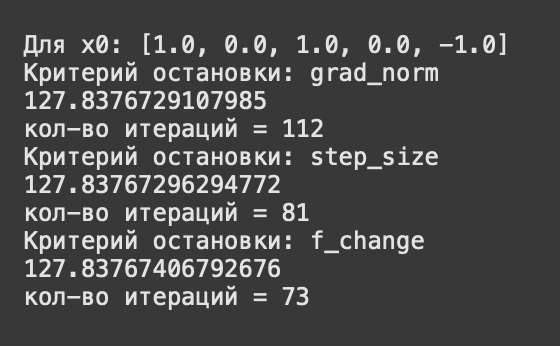
\includegraphics[width=0.8\textwidth]{stop3.png}
\end{center}
\end{frame}

\begin{frame}
\frametitle{ зависимость точности найденного решения от выбора критерия остановки}
\begin{center}
    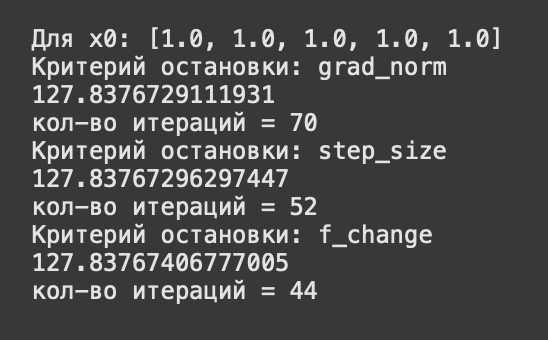
\includegraphics[width=0.8\textwidth]{stop4.png}
\end{center}
\end{frame}

\begin{frame}
\frametitle{ВЫВОД зависимость точности найденного решения от выбора критерия остановки}

Каждый критерий имеет свои преимущества и недостатки. Если требуется гарантированно добиться сходимости к стационарной точке, лучше использовать grad\_norm. Если важна экономия вычислительных ресурсов при достаточно быстром получении результата, можно предпочесть step\_size или f\_change.

Из проведенных экспериментов видно, что f\_change выглядит наиболее эффективным с точки зрения числа итераций.


\end{frame}
\end{document}